\documentclass[a4paper]{report}
%\documentclass[a4paper,twoside,openright]{report}
\usepackage[utf8]{inputenc}
\usepackage[T1]{fontenc}
\usepackage[ngerman,english]{babel}
\usepackage{titlesec}
\usepackage{subfigure}
\usepackage{graphicx}
\usepackage{parskip}
\usepackage{lmodern}
\usepackage{adjustbox}
\usepackage{tikz}
\usepackage{amsmath}
\usepackage{amssymb}
\usepackage{caption}

\usepackage{multirow}
\usepackage{listings}
\usepackage{xcolor}
\lstdefinestyle{promptstyle}{
    basicstyle=\ttfamily\small,
    breaklines=true,
    frame=none,
    backgroundcolor=\color{white},
    showstringspaces=false,
    columns=fullflexible,
    keepspaces=true,
    xleftmargin=1em,
    xrightmargin=1em
}
\usepackage{placeins}
\usepackage{algorithm}
\usepackage{algpseudocode}
\usepackage{pgfplots}
\usepackage{pdflscape}
\usepackage[hidelinks]{hyperref}
\usetikzlibrary{arrows,shapes,fit,positioning}
\usetikzlibrary{decorations.pathmorphing}
\usetikzlibrary{decorations.markings}

\pgfplotsset{compat=1.18}

\titleformat{\chapter}[display]
{\normalfont\huge\bfseries}{\chaptertitlename\ \thechapter}{20pt}{\Huge}

% configure autoref
\addto\extrasenglish{
	\def\chapterautorefname{Chapter}
	\def\subsectionautorefname{Subsection}
	\def\sectionautorefname{Section}
}

% this alters "before" spacing (the second length argument) to 0
\titlespacing*{\chapter}{0pt}{-50pt}{20pt}

\author{}
\date{\today}
\begin{document}
\pagestyle{empty}
\begin{titlepage}
\begin{center}
  % Upper part of the page  
	
\includegraphics[width=10cm,clip,trim=0 0 0 0\textwidth]{rptu}\\[2cm]
	% {
	% 	\linespread{1.5}\selectfont
	% 	\textsc{\LARGE Rheinland-Pfälzische Technische Universität Kaiserslautern-Landau}\\[0.5cm]
	% }
  \textsc{\large Fachbereich Informatik}\\[1.5cm]
	\vfill
  \textsc{\Large Master's Thesis}\\[0.5cm]
{
  \linespread{1.0}\selectfont
{\LARGE   \textsc{Creating and Benchmarking Learned Database Components using LLMs}\\[2cm]}
}

  { \Large
  Author:\\
	Preksha Rajesh Shah\\[2cm]
  {\small submitted on: \\
  \today}
  }\\[1cm]

  Supervisor\\
  Angjela Davitkova\\[1cm]
  Reviewers\\
  Prof. Dr.-Ing. Sebastian Michel\\

  
\end{center}
\end{titlepage}

%
\cleardoublepage


\begin{abstract}
Learned cardinality estimation has shown that neural networks can outperform traditional rule-based estimators, but training these models requires large volumes of labeled data obtained through expensive database query execution. This thesis presents a framework that combines large language model-based query generation with active learning to reduce this labeling cost. An LLM generates diverse SQL workloads from a given database schema, a four-layer validation pipeline filters invalid queries, and an active learning loop selects only the most informative queries for execution and labeling. The trained Multi-Set Convolutional Network achieves competitive estimation accuracy while requiring significantly fewer labeled queries than a fully supervised baseline. The entire pipeline is schema-agnostic and fully automated, enabling scalable training of learned database components on arbitrary relational schemas.
\end{abstract}

\cleardoublepage
\selectlanguage{english}

\tableofcontents
\thispagestyle{empty}
\listoffigures
\thispagestyle{empty}
\begingroup
\thispagestyle{empty}
\let\clearpage\relax
\vspace{3cm}
\listofalgorithms
\let\clearpage\relax
\vspace{3cm}
\listoftables
\endgroup
\thispagestyle{empty}


%%% 
%%% Add your inputs here
%%%

% !TEX root =  main.tex

\chapter{Introduction}
\label{chap:introduction}
\pagestyle{plain}
\setcounter{page}{1}

\section{Problem Statement}

Query optimization in relational databases depends heavily on cardinality estimation, which predicts how many rows a query will return before execution. Get the estimate right and the optimizer picks a fast and efficient execution plan. Incorrect estimates can lead to severely suboptimal execution plans and substantial performance degradation. Traditional estimators lean on assumptions like attribute independence and uniform value distributions that rarely hold in practice, and the resulting errors often compound across joins, leading to plans that are far from optimal.

Over the past few years, learned cardinality estimators have shown that neural networks can do a better job. The Multi-Set Convolutional Network (MSCN) by Kipf et al.~\cite{DBLP:conf/cidr/KipfKRLBK19} demonstrated that a relatively simple deep learning model can capture cross-table correlations that rule-based estimators miss entirely. But learned models come with their own cost: they need large quantities of labeled training data, and each label requires executing a query on a live database to record its true row count. On a complex schema this execution-based labeling can take hours, making it the dominant bottleneck in any pipeline that trains learned estimators from scratch.

Meanwhile, large language models have become remarkably good at generating SQL. Work like SQLStorm~\cite{DBLP:journals/pvldb/SchmidtLBN25} has shown that LLMs can produce diverse, realistic query workloads at scale when given a schema and a well-crafted prompt. But generating queries is only half the problem. Those queries still need to be executed to obtain labels, and that execution cost remains.

This thesis investigates whether large language models can be used to generate diverse SQL workloads while active learning selectively identifies the most informative queries for execution-based labeling. The goal is to train accurate learned cardinality estimators while significantly reducing the cost associated with labeling large query workloads.

\section{Proposed Approach}

In the proposed framework, the LLM acts as a workload generator rather than a runtime query component. Given a database schema, the model produces synthetic \texttt{SELECT COUNT(*)} queries that are subsequently validated, filtered, and encoded into the representation expected by MSCN. Instead of labeling the entire workload, active learning is used to identify informative queries based on model uncertainty. Only the selected queries are executed to obtain ground-truth cardinalities, after which the estimator is retrained iteratively on the expanded labeled set.

The whole process is packaged as a largely automated pipeline that is adaptable across supported relational schemas. Within the supported SQL fragment and available join metadata, the same pipeline can be applied to different database schemas without redesigning the overall workflow. A researcher provides a database schema and a small set of configuration parameters, after which the pipeline operates automatically. The pipeline generates queries, validates them through four filtering layers, labels the selected subset, trains the MSCN model, and outputs a full evaluation dashboard. The framework therefore minimizes the need for manual query engineering and supports automated workload generation, labeling, and training.

The motivation draws on two bodies of prior work. Wang et al.~\cite{DBLP:journals/pvldb/WangQWWZ21} showed that the diversity and structural properties of the training workload have a profound effect on learned estimator quality, and Davitkova and Michel~\cite{DBLP:journals/corr/abs-2512-20271} demonstrated that generative AI can automate the creation of training data for database components. We build on both: using LLMs for diverse workload generation and active learning for efficient labeling.

\section{Contributions}

This thesis makes four primary contributions. First, it presents an LLM-based workload generation framework for learned cardinality estimation capable of producing structurally diverse SQL query workloads. Second, it integrates active learning into the labeling pipeline and evaluates uncertainty-based acquisition strategies for reducing execution-based labeling cost. Third, it introduces an automated training pipeline that supports workload generation, validation, labeling, and estimator training for relational schemas with defined join relationships while reducing the amount of manual workload engineering required during training. Fourth, it provides an experimental evaluation on the IMDB benchmark analyzing workload diversity, labeling efficiency, and estimation performance under different workload and acquisition settings.
% !TEX root =  main.tex
\chapter{Background}
\label{chap:background}
\pagestyle{plain}

\section{Learned Database Systems and Cardinality Estimation}

Modern database systems rely on query optimizers to generate efficient execution plans. At the core of query optimization lies cardinality estimation, which predicts the number of tuples produced during intermediate stages of query execution\cite{HE2024102854}. These estimates directly influence join ordering, operator selection, and resource allocation. Inaccurate estimates can therefore lead to inefficient execution plans and substantial performance degradation. Traditional cardinality estimation techniques typically rely on statistical summaries such as histograms and sampling, together with assumptions including attribute independence and uniform value distributions. Although these methods are computationally efficient, they often fail to reflect real-world data characteristics. Real-world datasets frequently contain strong correlations across attributes and relations, particularly in join-heavy workloads with multiple predicates. Consequently, conventional techniques often produce inaccurate estimates for complex analytical queries.

Traditional cardinality estimation methods primarily rely on statistical summaries collected from database tables. One widely used technique involves histograms, where the value distribution of a column is approximated using a fixed number of buckets\cite{yi2025monomenhancingmonotonicitylearned}. Equi-width histograms divide the value domain into uniformly sized intervals, whereas equi-depth histograms attempt to maintain approximately equal numbers of tuples in each bucket. These summaries allow the optimizer to approximate predicate selectivity without scanning the underlying data. For example, under a uniformity assumption, the selectivity of an equality predicate can be estimated as:

\begin{equation}
|\sigma_{A=v}(R)| = \frac{|R|}{V(R,A)}
\end{equation}

where $|R|$ denotes the number of tuples in relation $R$, and $V(R,A)$ represents the number of distinct values in attribute $A$. Although computationally efficient, this approximation assumes that values are uniformly distributed and statistically independent, assumptions that rarely hold in practice.

The limitations of independence assumptions become particularly severe in join-heavy workloads. Traditional optimizers frequently estimate join cardinalities using simplified formulas based on value distributions of join attributes. A common approximation for an equi-join between relations $R$ and $S$ on attribute $A$ is:

\begin{equation}
|R \bowtie S| = \frac{|R| \cdot |S|}{\max(V(R,A),V(S,A))}
\end{equation}

This formulation assumes that join values are evenly distributed and statistically independent across relations. In practice, however, relational data often contains skewed distributions, hierarchical dependencies, and complex correlations that violate these assumptions. As query complexity increases, estimation errors may propagate through the execution plan and degrade query performance.

Another limitation of traditional approaches is their inability to adapt effectively to evolving workloads and changing data distributions. Modern database systems continuously ingest new records and experience shifting query patterns over time. Maintaining accurate statistical summaries under such conditions is computationally expensive, particularly for large-scale databases. As data distributions drift, previously collected statistics gradually become outdated, reducing estimation quality and leading to suboptimal query plans.

These limitations have motivated the development of learned database systems, where machine learning models replace or augment traditional statistical estimators. Instead of relying on handcrafted assumptions regarding independence and uniformity, learned models infer relationships directly from query workloads and observed execution behavior. Learned cardinality estimation has therefore emerged as one of the most actively studied areas within learned database systems, aiming to capture complex predicate interactions and provide more robust estimates across diverse query workloads.

\section{MSCN and Deep Learning-based Estimation}

Kipf et al. proposed the Multi-Set Convolutional Network (MSCN), an important advancement in learning-based cardinality estimation~\cite{DBLP:conf/cidr/KipfKRLBK19}. MSCN reformulates cardinality estimation as a supervised learning problem in which query result sizes are predicted directly from query structure representations.

Deep learning-based cardinality estimation approaches aim to overcome the limitations of traditional statistical techniques by learning complex relationships from query workloads and observed execution behavior\cite{10.1145/3725355}\cite{10.14778/3750601.3750699}. Unlike histogram-based methods that rely on assumptions, neural models can capture non-linear dependencies between predicates, correlations across attributes, and interactions between joined relations. This capability is particularly important for analytical workloads containing multiple joins and selective predicates that violate independence assumptions. By learning from large collections of executed queries, deep learning models can generalize beyond explicitly stored statistics and provide more robust cardinality predictions for unseen query patterns.

MSCN represents SQL queries as collections of sets, including tables, joins, and predicates. This design is motivated by the observation that SQL query components are inherently unordered. Since SQL query semantics are independent of predicate ordering, the model must preserve permutation invariance across query components.

The concept of permutation invariance is closely related to the Deep Sets framework. Given a set of elements $X = \{x_1, x_2, \dots, x_n\}$, a permutation-invariant function can be expressed as

\begin{equation}
f(X) = \rho \left( \sum_{x \in X} \phi(x) \right)
\end{equation}

where $\phi$ represents a learnable embedding function that transforms individual set elements into latent representations, and $\rho$ denotes a function that maps the aggregated representation to the final output. In MSCN, predicates, joins, and table features are first embedded independently and subsequently aggregated using pooling operations such as averaging. This architecture enables the model to process queries containing variable numbers of joins and predicates while preserving semantic equivalence across different query orderings.

A central component of MSCN is the use of sampled bitmaps to represent table-level information. Instead of relying exclusively on symbolic query features, the model incorporates materialized samples from database tables to provide additional information regarding predicate selectivity and local data distributions. During preprocessing, a fixed number of tuples are sampled from each table. For a given query predicate, the model generates a bitmap indicating which sampled tuples satisfy the condition. These bitmaps provide compact approximations of predicate selectivity and local data distributions, enabling the model to capture correlations that are difficult to represent through traditional statistical summaries alone.

Training neural cardinality estimators introduces additional challenges related to data distribution and optimization stability. Cardinality values frequently span several orders of magnitude, ranging from single tuples to millions of rows. Directly predicting raw cardinalities can therefore destabilize training and bias optimization toward large outputs. To address this issue, most learned estimators apply logarithmic normalization before training. A common normalization strategy is defined as

\begin{equation}
y_{\text{norm}} =
\frac{
\log(y) - \log(y_{\min})
}{
\log(y_{\max}) - \log(y_{\min})
}
\end{equation}

where $y$ denotes the true cardinality and $y_{\min}$ and $y_{\max}$ correspond to the minimum and maximum observed cardinalities in the training data. Logarithmic normalization compresses the output range and reduces impact of extreme outliers, thereby improving optimization stability during gradient-based learning.

These challenges motivate the need for diverse and representative training workloads in learned cardinality estimation systems. Neural cardinality estimators may overfit to the specific query distributions observed during training and struggle to generalize to unseen workloads. This problem becomes particularly severe under workload shifts, where future query patterns differ substantially from historical training data. Queries containing unseen join structures, rare predicates, or previously unobserved value ranges may produce inaccurate predictions even if the model performs well on validation datasets. 

Despite these challenges, deep learning-based approaches have demonstrated substantial improvements over traditional histogram-based estimators for complex query workloads. By leveraging representation learning, permutation-invariant architectures, and sampled data representations, models such as MSCN can capture structural dependencies within SQL queries that are difficult to model using handcrafted statistical assumptions.

\section{Workload Sensitivity and Challenges}

The performance of learned cardinality estimators depends not only on the underlying model architecture but also on the characteristics of the training workload. Wang et al.~\cite{DBLP:journals/pvldb/WangQWWZ21} provide a comprehensive analysis of how different query properties influence learned cardinality estimators. Their study demonstrates that factors such as predicate selectivity, join complexity, and workload diversity significantly affect estimation accuracy and model robustness.

An additional challenge in learned cardinality estimation concerns model generalization and overfitting. Neural cardinality estimators are typically trained on finite query workloads that cover only a subset of the possible query space. Although modern neural architectures are capable of learning complex relationships between predicates and joins, they may also memorize recurring workload patterns instead of learning representations that remain robust across varying query distributions. This issue becomes particularly problematic when training workloads contain repetitive query templates or narrow distributions of predicate values.

Overfitting in learned estimators differs from traditional overfitting problems commonly observed in standard machine learning tasks. In cardinality estimation, the model must generalize not only across different input values but also across structurally distinct SQL queries. Queries may vary in the number of joins, predicate combinations, selectivity characteristics, and table interactions. Consequently, a model that performs well on validation data drawn from the same workload distribution may still fail when exposed to previously unseen query structures during deployment.

A major source of generalization difficulty is the combinatorial nature of relational query spaces. Even relatively small schemas can produce enormous numbers of distinct query structures through different combinations of joins and predicates. Since it is infeasible to observe every possible query during training, learned estimators must infer broader structural patterns from limited examples. This requirement further emphasizes the importance of representation learning and workload diversity.

Another challenge arises from the long-tailed distribution of query cardinalities. Real-world workloads frequently contain many moderately selective queries alongside a smaller number of highly selective or extremely broad scans. Neural models optimized primarily for average-case performance may therefore underperform on rare edge cases that appear infrequently during training.

Regularization techniques play an important role in improving model generalization. Methods such as dropout, early stopping, and weight decay reduce the risk of memorizing narrow workload patterns. In particular, dropout introduces stochasticity during training by randomly disabling subsets of neurons, encouraging the model to learn more robust distributed representations. Nevertheless, workload diversity remains one of the most important factors influencing generalization performance.

These challenges highlight an important distinction between learned cardinality estimation and traditional statistical approaches. While histogram-based methods rely on explicit assumptions regarding value distributions, neural estimators depend fundamentally on their ability to generalize from observed workloads to unseen query patterns. Consequently, understanding and improving generalization behavior remains a central research challenge in learned database systems.

\section{LLM-based SQL Generation and Generative AI for Database Systems}

Large language models (LLMs) have recently emerged as promising tools for structured query generation. The SQLStorm framework proposed by Schmidt et al.~\cite{DBLP:journals/pvldb/SchmidtLBN25} demonstrates that schema-aware prompting strategies can be used to generate large, diverse SQL query workloads. Unlike traditional template-based or rule-based query generation methods, LLMs are capable of producing structurally varied queries that better capture the diversity of real-world workloads.

A key advantage of LLM-based query generation is the ability to incorporate semantic information about database schemas. By conditioning on table structures, column names, and schema relationships, LLMs can generate queries that are both syntactically valid and semantically meaningful. This capability is particularly useful for complex schemas where manually constructing diverse workloads becomes difficult and time-consuming. Compared to manually engineered query templates, LLMs can additionally produce broader combinations of predicates, joins, and filtering conditions, enabling more diverse exploration of the query space.

LLM-generated workloads are especially relevant for learned database systems because they enable scalable creation of synthetic training queries beyond existing benchmark workloads. Such generated workloads may expose learned models to previously unseen query structures, predicate combinations, and join patterns, potentially improving workload diversity and model generalization.

Recent work by Davitkova and Michel~\cite{DBLP:journals/corr/abs-2512-20271} further explores the use of generative AI for automating data generation in learned database systems. Their framework proposes a structured pipeline in which query generation, validation, execution, and model training are integrated into a unified workflow. Generated queries are validated against the target schema to ensure syntactic and semantic correctness before being incorporated into the training process. The work additionally highlights the importance of schema-aware prompting and iterative refinement strategies for improving workload quality and diversity.

Despite these advances, generated queries must still be executed against the database in order to obtain ground-truth labels for supervised learning. Although query generation becomes automated, execution-based labeling remains computationally expensive and continues to limit scalability for learned cardinality estimation systems. This limitation motivates the exploration of approaches that reduce labeling cost while still maintaining workload diversity and estimator quality.

\section{Active Learning and Uncertainty Estimation}

Learned cardinality estimation systems require large quantities of labeled training data in order to generalize effectively across diverse query workloads~\cite{DBLP:conf/cidr/KipfKRLBK19,DBLP:journals/pvldb/WangQWWZ21}. However, obtaining ground-truth labels is computationally expensive because each query must be executed against the database to determine its true cardinality\cite{DBLP:phd/dnb/Woltmann23}. Active learning addresses this challenge by selectively choosing informative samples for labeling instead of exhaustively labeling entire query workloads~\cite{DBLP:journals/tnn/LiWCJDO25}.

A widely used active learning strategy is uncertainty sampling, where the model prioritizes samples for which it is least confident~\cite{DBLP:journals/tnn/LiWCJDO25}. In neural networks, predictive uncertainty can be estimated using Monte Carlo (MC) dropout. Understanding MC dropout first requires examining the role of standard dropout as a regularization technique\cite{DBLP:conf/cvpr/ZeeviSLSO25}.

Dropout was introduced as a regularization technique to reduce overfitting by randomly disabling units during training~\cite{srivastava2014dropout}. Baldi and Sadowski~\cite{DBLP:conf/nips/BaldiS13} analyzed its averaging and regularizing properties, showing that dropout discourages co-adaptation and can be interpreted as approximating an ensemble of subnetworks that share parameters.
 
Gal and Ghahramani~\cite{DBLP:conf/icml/GalG16} later demonstrated that retaining dropout during inference allows neural networks to approximate Bayesian inference. Instead of producing a single deterministic prediction, the model performs multiple stochastic forward passes using different dropout masks. The resulting distribution of predictions provides an approximate estimate of epistemic uncertainty, where higher predictive variance indicates greater uncertainty caused by limited training knowledge.

In learned cardinality estimation, MC dropout enables the identification of queries for which the estimator is uncertain. Queries associated with high predictive variance may contain patterns that are underrepresented in the training workload or difficult for the model to generalize. These uncertainty estimates therefore provide a principled mechanism for selecting informative queries during active learning.

Beyond uncertainty-based acquisition, active learning can additionally incorporate diversity-aware sampling strategies~\cite{DBLP:journals/tnn/LiWCJDO25}. Diversity-based selection encourages broader coverage of the query space by reducing redundancy among selected queries and exposing the model to a wider range of join structures, predicate combinations, and selectivity patterns. Balancing uncertainty-driven acquisition with broad workload coverage is important for improving model generalization across unseen workloads.

A practical limitation of MC dropout is the additional computational overhead introduced by repeated inference passes. Recent work by Srinivasan~\cite{Srinivasan2025Efficient} addresses this limitation through a model-splitting approach that separates deterministic and stochastic network components. When dropout is applied only after an initial deterministic portion of the network, the deterministic body can be executed once while the stochastic head is evaluated multiple times. This idea motivates more efficient use of MC dropout for uncertainty estimation in large candidate pools.

The integration of active learning with synthetic workload generation is particularly attractive for learned database systems. Large language models can efficiently generate large pools of candidate SQL queries~\cite{DBLP:journals/pvldb/SchmidtLBN25}, while recent work has also explored generative models for synthesizing training data for learned database components~\cite{DBLP:journals/corr/abs-2512-20271}. Active learning can then reduce the execution cost required to label these generated queries. Together, these approaches provide a scalable framework for improving data efficiency in learned cardinality estimation pipelines.

\section{Data Diversity and Distributional Similarity}

Diversity within synthetic workloads plays an important role in improving model generalization for learned database systems. The PAARS framework~\cite{DBLP:journals/corr/abs-2503-24228} explores persona-driven prompting strategies to encourage greater variation in generated query distributions. By varying prompting contexts and generation behavior, such approaches aim to produce workloads that better capture heterogeneous query patterns.

In order to test the quality of the generated data, the PAARS framework uses the KL divergence as a similarity metric between the generated data and real-world data. The KL divergence is a measure of the dissimilarity between two probability distributions, which can be used to test the similarity between the generated data and real-world data, especially in the case of SQL queries\cite{DBLP:journals/corr/abs-2512-20271}.

In the context of SQL query generation, KL divergence may be applied to workload characteristics such as join counts, predicate types, and selectivity distributions. Comparing these feature distributions provides a quantitative mechanism for evaluating whether synthetic workloads reflect structural properties commonly observed in real query traces. Such distributional analysis is particularly useful when assessing the realism and diversity of generated workloads used for training learned cardinality estimators.
\chapter{Related Work}
\label{chap:relatedwork}
\pagestyle{plain}

\section{Learned Cardinality Estimation}

Machine learning-based approaches for replacing traditional database components have gained significant attention, particularly in the context of cardinality estimation. A foundational contribution in this area is the Multi-Set Convolutional Network (MSCN) proposed by Kipf et al.~\cite{DBLP:conf/cidr/KipfKRLBK19}, which reformulates cardinality estimation as a supervised learning problem. Unlike conventional estimators that rely on simplifying assumptions such as attribute independence, MSCN represents queries as sets of tables, joins, and predicates, enabling the model to capture complex correlations across query components.

MSCN demonstrated that learned models could substantially outperform traditional histogram-based estimators on complex analytical query workloads.
Its permutation-invariant architecture and use of sampled bitmap representations enabled improved modeling of complex correlations across joins and predicates,
establishing MSCN as a foundational baseline for subsequent learned cardinality estimation research.

Despite these advantages, MSCN fundamentally depends on execution-based labeling. Each training instance requires executing a query on a database to obtain its true cardinality. This introduces substantial computational overhead and limits scalability, particularly when large and diverse workloads are required. Moreover, adapting to new schemas or workloads necessitates additional query execution, further increasing the cost. These limitations highlight a central challenge in learned cardinality estimation: the dependency on labeled data generated through expensive query execution.

\section{Workload Characteristics and Model Generalization}

Beyond model architecture, the effectiveness of learned cardinality estimators is strongly influenced by the characteristics of the training workload. Wang et al.~\cite{DBLP:journals/pvldb/WangQWWZ21} demonstrate that learned models are highly sensitive to factors such as predicate types, selectivity, join complexity, and query structure.

Their findings show that models trained on narrow or biased workloads often struggle to generalize to unseen query patterns. In particular, learned estimators may experience substantial performance degradation when evaluated on workloads containing predicate types, selectivity ranges, or join structures that differ from those observed during training.

The issue of workload shift further complicates deployment. In real-world systems, query distributions evolve over time, leading to discrepancies between training and inference workloads. Under such conditions, learned models can exhibit significant decreases in estimation accuracy. These observations emphasize the importance of constructing training datasets that are both diverse and representative of real-world query patterns.

Recent work on robust cardinality estimation under changing and evolving workloads~\cite{DBLP:journals/pvldb/NegiWKTMMKA23} further highlights the importance of adaptability, reinforcing the need for scalable data generation approaches capable of capturing a broad range of query characteristics.

\section{LLM-based SQL Workload Generation}

The emergence of large language models (LLMs) has introduced new possibilities for SQL workload generation. The SQLStorm framework~\cite{DBLP:journals/pvldb/SchmidtLBN25} demonstrates that LLMs can generate large-scale, diverse, and realistic SQL queries using schema-aware prompting techniques.

Unlike traditional template-based approaches, which are inherently limited in structural diversity, LLM-based methods can generate queries with varying levels of complexity, including different join structures, predicate combinations, and nested queries. This flexibility enables the creation of more realistic workloads that better reflect real-world usage patterns and expose learned models to broader query distributions.

Recent advances in text-to-SQL and structured reasoning further support the broader applicability of LLMs for SQL generation tasks. Systems such as CHASE-SQL~\cite{DBLP:conf/iclr/PourrezaL0CTKGS25} and TAPEX~\cite{DBLP:conf/iclr/LiuCGZLCL22} demonstrate that neural models are increasingly capable of understanding relational schemas, table structures, and complex query semantics. Evaluation studies by Rahaman et al.~\cite{DBLP:conf/edbt/RahmanZMCP25} additionally highlight both the strengths and limitations of contemporary LLMs in structured query generation settings.

However, existing LLM-based approaches primarily focus on query generation rather than labeled data creation. Generated queries must still be executed against the database in order to obtain ground-truth cardinalities, thereby retaining the dependency on execution-based labeling and limiting scalability for learned cardinality estimation pipelines.

Furthermore, existing LLM-based approaches evaluate their models on externally curated benchmark workloads rather than on LLM-generated queries. In contrast, the approach presented in this thesis supports a self-contained pipeline in which LLM-generated queries are used for training and validation in LLM-based runs, while controlled comparisons may additionally use synthetic workloads for reproducibility.

\section{Generative AI for Training Database Components}

Recent work on integrating generative AI into database systems has sought to address the limitations of manual and execution-based data generation. Davitkova and Michel~\cite{DBLP:journals/corr/abs-2512-20271} propose a framework that leverages generative models to automate the training of learned database components.

Their framework introduces a structured pipeline that integrates query generation, validation, execution, and model training. By automating query generation, it reduces reliance on manually collected query logs and enables the creation of diverse training datasets. Techniques such as schema-aware prompting and iterative refinement are further used to improve the quality and realism of generated queries.

Despite these advancements, generated queries must still be executed to obtain ground-truth cardinalities for supervised training. Consequently, query execution continues to represent a significant computational cost within learned cardinality estimation pipelines.

\section{Active Learning and Uncertainty Quantification}

Active learning provides a complementary approach to improving data efficiency in supervised learning systems. A recent survey on deep active learning~\cite{DBLP:journals/tnn/LiWCJDO25} describes how active learning methods aim to reduce labeling requirements by selecting informative samples for annotation. A core mechanism for this selection is uncertainty quantification, which allows a model to identify the inputs it is least confident about.

A theoretically grounded method for estimating neural network uncertainty is Monte Carlo (MC) dropout. The regularizing and averaging properties of dropout were fundamentally established by Baldi and Sadowski~\cite{DBLP:journals/ai/BaldiS14}, who demonstrated that dropout acts as a computationally efficient approximation of an exponentially large ensemble of subnetworks. By retaining dropout during inference and performing multiple stochastic forward passes, models can approximate predictive uncertainty, with variation across predictions often used as an estimate of epistemic uncertainty~\cite{DBLP:conf/icml/GalG16}\cite{hossain2026uatliteinferencetimeuncertaintyawareattention}.

While MC dropout provides useful approximate uncertainty estimates, its repeated forward passes introduce substantial computational overhead\cite{hossain2026uatliteinferencetimeuncertaintyawareattention}. This issue is particularly problematic when querying large unlabeled pools during active learning. To address this, Srinivasan~\cite{Srinivasan2025Efficient} recently explored model-splitting techniques that partition the network into a deterministic body and a stochastic head. This architectural optimization achieves up to a 25\--33x speedup in inference, transforming MC dropout from a theoretically appealing concept into a highly practical tool for rapid uncertainty quantification.

In the context of learned cardinality estimation, active learning can be used to minimize the number of queries that need to be executed for expensive labeling. Prior work on active learning for ML-enhanced database systems has shown that additional query labels can be collected cost-effectively to improve deployed model performance~\cite{DBLP:conf/sigmod/MaDDS20}. By prioritizing queries where the model is uncertain or performs poorly, it is possible to achieve high estimation accuracy with fewer labeled samples.

In addition to uncertainty-based strategies, diversity-based sampling plays an important role in ensuring that selected queries cover a wide range of patterns. This is particularly relevant when working with synthetically generated data, where redundancy may otherwise reduce training effectiveness. Combining uncertainty and diversity criteria allows for the construction of efficient and representative training datasets.

While active learning is well established within machine learning research, its use in learned database systems has received comparatively limited research attention. Integrating active learning with LLM-based query generation provides a practical and scalable mechanism for improving labeling efficiency in learned cardinality estimation systems.

\section{Data Diversity and Distribution Alignment}

Ensuring that synthetic workloads reflect real-world query distributions is important for training robust learned database systems. The PAARS framework~\cite{DBLP:journals/corr/abs-2503-24228} explores persona-based generation strategies to encourage greater variation in generated data distributions and improve workload diversity.

A key contribution of this work is the use of KL divergence to measure similarity between generated and real-world data distributions. This provides a quantitative mechanism for evaluating whether synthetic workloads capture important structural characteristics of observed query patterns. In the context of SQL workloads, such metrics can be applied to distributions over query features including join counts, predicate types, and selectivity ranges.

Distribution alignment is particularly important for learned cardinality estimation because models trained on unrealistic synthetic workloads may fail to generalize effectively to real query patterns. Incorporating distributional similarity metrics into workload generation therefore helps improve both dataset diversity and representativeness.

\section{Positioning of the Proposed Approach}

The existing literature demonstrates significant recent progress in learned database systems and LLM-based data generation. Models such as MSCN~\cite{DBLP:conf/cidr/KipfKRLBK19} highlight the potential of learned approaches for cardinality estimation, while studies on workload characteristics~\cite{DBLP:journals/pvldb/WangQWWZ21} emphasize the importance of diverse and representative training data. LLM-based frameworks such as SQLStorm~\cite{DBLP:journals/pvldb/SchmidtLBN25} and generative pipelines~\cite{DBLP:journals/corr/abs-2512-20271} further demonstrate the practical feasibility of scalable SQL workload generation.

However, a common limitation across these approaches is the continued reliance on execution-based labeling. Although query generation has become increasingly automated, obtaining ground-truth labels still requires executing queries on a database, introducing substantial computational overhead.

The approach proposed in this thesis addresses this limitation by leveraging LLMs to generate diverse SQL workloads while using active learning to minimize the number of expensive database executions required for labeling. Rather than eliminating execution-based supervision entirely, the framework is designed to reduce labeling cost by selecting informative queries for execution and training. Furthermore, by incorporating active learning~\cite{DBLP:journals/tnn/LiWCJDO25} and diversity-aware generation strategies~\cite{DBLP:journals/corr/abs-2503-24228}, the proposed method aims to improve both data efficiency and workload representativeness.

Within the proposed framework, the LLM acts as a workload generator, while the trained supervised model serves as the final learned database component during inference. This separation enables scalable training workflows and supports more efficient development of learned cardinality estimation systems.

The primary contribution of this work does not lie in the introduction of a novel neural architecture for cardinality estimation, but rather in the design and evaluation of an automated training framework that integrates LLM-based workload generation with uncertainty-guided active learning. The proposed approach specifically addresses the practical challenges associated with execution-based labeling by reducing the number of required database executions while maintaining workload diversity and estimation quality. In this context, the thesis investigates how automated workload generation and active learning strategies can improve the scalability and data efficiency of training learned cardinality estimation systems.
% !TEX root =  main.tex
\chapter{Approach}
\label{chap:approach}
\pagestyle{plain}

This chapter describes the proposed framework for training learned cardinality estimators using LLM-generated workloads and active learning. First, the overall system architecture and workflow are presented. The chapter then discusses key pipeline properties including modularity, schema independence, reliability, and reproducibility.

Effective training of a learned cardinality estimator requires balancing two conflicting requirements: the availability of a large, diverse set of labeled queries and the practical constraints associated with obtaining such labels. Each label demands executing a query on a live database, which is slow and expensive. The proposed framework addresses this challenge by integrating query generation, labeling, feature extraction, active learning, and evaluation into a unified workflow.

\section{System Architecture}

The system integrates four stages into a largely automated workflow, with environment-specific setup (database access, model runtime, and schema artifacts) handled before execution. Figure~\ref{fig:Pipeline} illustrates how data flows from the database schema to the trained estimator and evaluation outputs.

\begin{figure}[tbp]
\centering

\includegraphics[width=\textwidth]{Report/graphs/pipeline.png}
\caption{Overview of the Proposed End-to-End Pipeline}
\label{fig:Pipeline}
\end{figure}

The pipeline begins with query generation. The database schema and column statistics are provided to a large language model, which generates batches of \texttt{SELECT COUNT(*)} queries representing diverse analytical workloads. The generated queries contain varying join structures, predicate combinations, and selectivity patterns. For environments where LLM-based generation is impractical, the framework also supports a deterministic synthetic query generator. Chapter~\ref{chap:query_generation} explains the prompt design, diversity mechanisms, and the comprehensive four-layer validation process used to detect malformed or unsupported queries before they are executed.

Validated queries are then labeled by executing them against PostgreSQL to obtain ground-truth cardinalities. For each query, the framework reconstructs a corresponding \texttt{SELECT COUNT(*)} statement and records the returned row count. Query execution represents the most computationally expensive stage of the pipeline, particularly for complex join queries and large workloads. This execution cost motivates the integration of active learning to reduce the number of queries requiring labeling.

Before training, each query is converted into a fixed-size tensor representation for neural processing. Each query is decomposed into tables, predicates, and joins. Individual elements are encoded using one-hot vectors and bitmap representations indicating which sampled rows satisfy the query predicates. These bitmaps capture data distributions together with query structure. The complete encoding process and MSCN architecture are described in Chapter~\ref{chap:training_approach}.

The active learning loop integrates model training, query selection, and labeling into a single iterative workflow. Training begins with a small randomly labeled seed set used to initialize the MSCN model. After the initial training phase, the model evaluates the remaining unlabeled queries, and the acquisition function ranks candidate samples according to the selected acquisition strategy. The highest-ranked queries are then executed to obtain ground-truth labels and incorporated into the training set before the model is retrained.

The framework implemented in this work supports three acquisition strategies: random sampling and MC Dropout variance-based sampling. These strategies represent different trade-offs between acquisition overhead and label efficiency. These strategies represent different trade-offs between computational overhead and labeling efficiency. A detailed discussion of the active learning framework, acquisition functions, and experimental configuration is presented in Chapter~\ref{chap:active_learning}.


\section{Pipeline Properties}

Several properties distinguish the proposed framework from earlier approaches to learned cardinality estimation. The pipeline is designed to operate across relational schemas containing defined foreign-key relationships. Given table definitions, column types, and join relationships, the framework automatically generates queries, validates them, extracts features, and trains the estimator without requiring workload-specific query engineering or benchmark-specific preprocessing. Consequently, the same implementation can be adapted to different database schemas without modifications to the overall pipeline structure. This portability is important because learned cardinality estimators must be retrained efficiently as schemas and workloads evolve over time.

Each stage of the pipeline is implemented as an independent component with clearly separated responsibilities. For example, the query generation module can be configured to use different large language models or alternative generation mechanisms, such as rule-based or template-based approaches, without requiring modifications to the remaining stages of the pipeline. Similarly, both the acquisition strategy used during active learning and the neural network architecture employed for estimation can be replaced independently. This modular design supports controlled experimentation by allowing individual components to be evaluated in isolation.

The framework additionally incorporates mechanisms to ensure reliable execution during large-scale processing. Queries that exceed the execution time limit are retried using a back-off strategy, while queries that continue to fail after all retry attempts are discarded from the final labeled workload. Rollback and cleanup procedures ensure that failed executions do not affect subsequent queries. As a result, the system can process large workloads with minimal manual intervention while preserving the quality of collected supervision signals.

The framework also incorporates several mechanisms to improve experimental reproducibility. Random seeds are consistently applied across Python, NumPy, and PyTorch in order to reduce nondeterministic behavior during training. Furthermore, all hyperparameters are logged alongside experimental outputs, and timestamped result directories prevent runs from accidentally overwriting previous results.
% !TEX root =  main.tex
\chapter{Query Generation Approach}
\label{chap:query_generation}
\pagestyle{plain}

A learned cardinality estimator is only as effective as the query workload used during training. If the model is trained on a narrow and repetitive set of queries, it is more likely to memorize recurring patterns than to learn representations that generalize effectively to unseen workloads. In contrast, training on structurally diverse queries that cover a broad range of join topologies, predicate selectivities, and table combinations provides a stronger foundation for accurate estimation across different query distributions. This chapter describes the workload generation process used in this work, beginning with query generation through a large language model and followed by a deterministic fallback mechanism. It also explains the validation procedures that ensure every query entering the training pipeline is syntactically correct, compatible with the database schema, and properly formatted for downstream processing.

Importantly, the generated workload serves a dual purpose. It provides both the training pool from which active learning selects queries for labeling and the held-out validation set used to evaluate the trained estimator. Unlike prior approaches that generate queries solely for training while relying on separate benchmark workloads for evaluation, the proposed pipeline uses LLM-generated queries throughout both training and evaluation. As a result, the evaluation remains self-contained and independent of externally curated test workloads.


\section{Why Use a Language Model}

The traditional alternatives for obtaining training queries each have clear drawbacks. Query logs drawn from production systems carry privacy risks and tend to reflect the habits of a particular user base rather than the full space of possible queries. Template-based generators can produce any structure their templates define, but those templates must be written by hand and rarely capture the subtle correlations and predicate distributions found in real workloads. Uniform random sampling over the schema produces syntactically valid queries but distributes predicates and join patterns in ways that bear little resemblance to actual usage.

Large language models address many of these limitations effectively. Models such as Llama 3.2 are trained on extensive corpora of source code, technical documentation, and natural language text that contain substantial amounts of SQL and database-related content. Consequently, they are capable of generating syntactically correct and semantically meaningful SQL queries when provided with schema information and generation constraints. Prior work shows broad SQL-generation capability, but in this implementation generation is intentionally constrained to a subset compatible with downstream encoding: SELECT COUNT(*), bounded table count, valid join paths, and conjunctive comparison predicates \cite{DBLP:journals/corr/abs-2512-20271}.

The generated workloads are not limited to fixed templates or manually enumerated query patterns. Instead, the diversity arises from the model’s learned representation of SQL syntax and query semantics, enabling the generation of structurally varied workloads that remain compatible with the underlying schema. Previous studies further demonstrate that large language models can adapt query generation to different workload requirements and database contexts while preserving both syntactic and semantic correctness \cite{DBLP:journals/corr/abs-2512-20271}. This capability is particularly important for learned cardinality estimation, where training effectiveness depends strongly on exposure to a broad and representative range of query patterns.

\section{Prompt Design}

The quality of the generated workload depends strongly on the prompt design. Ours is structured as a five-part template, illustrated in Figure~\ref{fig:prompt_structure}. The first part assigns a role: \begin{lstlisting}[
    style=promptstyle,
    caption={LLM prompt template (excerpt)},
    label={lst:prompt}
]
            You are a SQL query workload generator for a database.
\end{lstlisting} This framing primes the model to produce queries rather than explanations or tutorials. The second part injects the full database schema as DDL statements table names, columns, data types, foreign keys so the model knows what it is allowed to reference. The third part supplies column statistics: minimum and maximum values for numeric columns, which help the model pick predicate values that fall within realistic ranges rather than generating unrealistic values. The fourth part defines the structural constraints imposed on generated queries, while the fifth part specifies the required output format for downstream parsing and processing.

\begin{figure}[tb]
\centering
\begin{tikzpicture}[
    block/.style={draw, rectangle, rounded corners=3pt, minimum width=12cm, minimum height=1.3cm, text centered, font=\small},
    arrow/.style={->, thick, >=stealth},
    node distance=1.5cm
]
    \node [block, fill=blue!15] (role) {\textbf{1. Role Assignment}: ``You are a SQL query workload generator for a database.''};
    \node [block, fill=green!15, below=of role] (schema) {\textbf{2. Schema Context}: Complete DDL with table names, columns, types, and relationships};
    \node [block, fill=yellow!15, below=of schema] (stats) {\textbf{3. Column Statistics}: Min/max values and cardinalities for numeric columns};
    \node [block, fill=orange!15, below=of stats] (rules) {\textbf{4. Generation Rules}: Strict constraints on query structure and complexity};
    \node [block, fill=red!15, below=of rules] (output) {\textbf{5. Output Format}: JSON array specification with example queries};

    \draw [arrow] (role) -- (schema);
    \draw [arrow] (schema) -- (stats);
    \draw [arrow] (stats) -- (rules);
    \draw [arrow] (rules) -- (output);

    \node [left=0.3cm of role, font=\scriptsize, text=gray, rotate=90, anchor=south] {Context};
    \node [left=0.3cm of rules, font=\scriptsize, text=gray, rotate=90, anchor=south] {Constraints};

\end{tikzpicture}
\caption{Five-part prompt template. The upper components provide schema and statistical context, while the lower components define structural generation constraints.}
\label{fig:prompt_structure}
\end{figure}

The fourth component introduces constraints motivated by the requirements of the downstream Multi-Set Convolutional Network (MSCN) encoder, introduced in Section 2.2 and discussed in detail in Section 7.3. More broadly, however, similar restrictions are common across supervised learned cardinality estimators, since such models rely on fixed and well-defined feature representations of SQL queries. The subset of SQL supported by the system is therefore determined not by arbitrary implementation preferences, but by the expressive limitations of the encoding scheme and the neural architecture operating on top of it. Queries that cannot be represented consistently in feature space cannot be processed reliably during either training or inference.

For this reason, every generated query is required to follow a constrained SQL fragment compatible with the MSCN representation. Each query must use \texttt{SELECT COUNT(*)}, involve between one and three tables with proper aliases, join tables only through valid foreign key relationships defined in the schema, and restrict filter predicates to simple comparison operators such as \texttt{=}, \texttt{<}, and \texttt{>}, connected exclusively through conjunctions using \texttt{AND}. More complex SQL constructs including \texttt{OR}, \texttt{IN}, \texttt{LIKE}, nested subqueries, aggregations, and other advanced operators are intentionally excluded from the workload. These constructs cannot be encoded correctly by the MSCN feature representation and would therefore produce incomplete or misleading input features. Enforcing these constraints during query generation ensures that every query entering the training pipeline remains schema-compatible, representable by the encoder, and valid for downstream model training and evaluation.

The fifth component of the prompt specifies the output format as a JSON array, where each element contains a single key, "sql", whose value is a complete SQL query generated by the language model. This structured representation ensures reliable and deterministic parsing of the model output. In cases where the model produces additional explanatory text alongside the JSON, a lightweight post-processing step based on regular expressions is applied to extract the valid JSON content.


\section{Workload Diversity}

When used iteratively for data generation, large language models can gradually lose diversity, producing outputs that concentrate on a narrower set of patterns over time. This behavior aligns with the phenomenon of model collapse~\cite{collapse}, where repeated sampling or self-conditioned generation reduces distributional coverage and overemphasizes high-probability outputs. In the context of SQL workload generation, this appears as recurring join structures and similar predicate configurations across batches.

To address this issue, we introduce a rotating set of diversity hints that guide the model toward different regions of the query space. Five emphasis hints cycle in sequence to rebalance generation toward underrepresented query patterns while preserving a weighted structural mix ( simple and medium-complexity queries) and practical labeling cost. The hints emphasize single-table queries, medium-complexity joins involving two to three tables, mixed point and range predicates, and selectivity extremes ranging from highly selective filters to broad scans.

These categories are motivated by prior work on learned cardinality estimation, which shows that model performance depends strongly on the structural and statistical properties of the training workload. In particular, the number of joined tables influences query complexity, predicate types affect selectivity estimation, and the distribution of cardinalities, especially the inclusion of extreme values-plays an important role in model calibration and generalization~\cite{DBLP:conf/cidr/KipfKRLBK19}. By explicitly targeting these aspects, the proposed hint rotation encourages coverage of both common query patterns and less frequent edge cases. Advancing the hint index with each batch further helps maintain a balanced distribution across categories, improving the overall diversity and representativeness of the generated workload.

Generating all queries within a single prompt would exceed the model's context window and reduce workload diversity. Instead, the system works in batches. The total query target is divided by the batch size, and each batch gets a fresh prompt with the current diversity hint. Algorithm~\ref{alg:batch_generation} outlines the procedure.

\begin{algorithm}[tb]
\caption{LLM-Based Query Generation}
\label{alg:batch_generation}
\begin{algorithmic}[1]
\Require target\_count
\Ensure query\_set

\State query\_set $\gets \emptyset$
\State num\_batches $\gets$ compute\_batches(target\_count)

\For{each batch in num\_batches}
    \State hint $\gets$ select\_diversity\_hint($|$query\_set$|$)
    \State prompt $\gets$ construct\_prompt(schema, statistics, hint)

    \For{$attempt \gets 1$ to $n$}
        \State response $\gets$ LLM(prompt)
        \State queries $\gets$ extract\_valid\_SQL(response)
        
        \If{queries $\neq \emptyset$}
            \State query\_set $\gets$ query\_set $\cup$ queries
            \State \textbf{break}
        \EndIf
    \EndFor
\EndFor

\State \Return trim(query\_set, target\_count)
\end{algorithmic}
\end{algorithm}

The algorithm generates a set of SQL queries using a large language model (LLM) until a target count is reached. It first determines the number of batches required and initializes an empty query set. For each batch, a diversity hint is selected based on the number of queries generated so far, encouraging variation in query structure and complexity. A prompt is then constructed using the database schema, column statistics, and the selected hint. To improve robustness, the algorithm allows up to three attempts per batch. In each attempt, the prompt is sent to the LLM, and the response is parsed to extract valid SQL queries. If at least one valid query is obtained, the queries are added to the collection and the algorithm proceeds to the next batch. This retry mechanism helps handle cases where the model produces invalid or unparseable output. After processing all batches, the collected queries are trimmed to match the exact target count. This ensures that the final output is both size-constrained and diverse, making it suitable for downstream training tasks.

Due to the stochastic nature of large language model inference, individual generation requests may fail in several ways, including network or API errors, malformed or non-JSON responses, or outputs that do not conform to the expected SQL structure. In this context, a call refers to a single request to the language model for generating a batch of queries. To improve robustness, each batch generation request is retried up to three times if no valid queries can be extracted from the response. The retry limit of $n=3$ was selected as a practical compromise between robustness and runtime overhead. Empirically, most batches already succeed on the first attempt, while one or two additional retries recover nearly all remaining failures. Increasing the retry limit further was observed to provide only marginal improvements while unnecessarily increasing generation latency. In practice, this retry strategy achieves a near-perfect batch-level success rate, meaning that almost every batch eventually produces at least one valid, schema-compliant SQL query.


\section{Query Validation Pipeline}

Even with careful prompting, some fraction of the LLM's output will be unusable. A query might reference a column that does not exist, use an \texttt{OR} that slipped past the instructions, or simply be unparseable. Rather than trusting the LLM to be perfect, we pass every query through four progressively stricter validation layers, illustrated in Figure~\ref{fig:validation_pipeline}.

\begin{figure}[htbp]
\centering
\begin{tikzpicture}[
    node distance=1.8cm,
    block/.style={draw, rectangle, rounded corners=3pt, minimum width=5.5cm, minimum height=1.1cm, align=center, font=\small},
    reject/.style={draw, rectangle, rounded corners=3pt, minimum width=2.5cm, minimum height=0.8cm, align=center, font=\small, fill=red!15},
    arrow/.style={->, thick, >=stealth},
    rarrow/.style={->, thick, >=stealth, red!70},
]
    \node [block, fill=gray!15] (raw) {Raw LLM Output (N queries)};
    \node [block, fill=blue!15, below=of raw] (struct) {Layer 1: Structural Validation\\{\scriptsize Regex-based keyword filtering}};
    \node [block, fill=green!15, below=of struct] (parse) {Layer 2: SQL Parsing\\{\scriptsize FROM/WHERE clause extraction}};
    \node [block, fill=yellow!15, below=of parse] (schema) {Layer 3: Schema Validation\\{\scriptsize Table/column existence checks}};
    \node [block, fill=orange!15, below=of schema] (format) {Layer 4: Format Conversion\\{\scriptsize MSCN-compatible structure}};
    \node [block, fill=green!30, below=of format] (valid) {Valid Queries ($\leq$ N)};

    \draw [arrow] (raw) -- (struct);
    \draw [arrow] (struct) -- (parse);
    \draw [arrow] (parse) -- (schema);
    \draw [arrow] (schema) -- (format);
    \draw [arrow] (format) -- (valid);

    \node [reject, right=2.5cm of struct] (r1) {Reject: Forbidden\\keywords found};
    \node [reject, right=2.5cm of parse] (r2) {Reject: Parse\\failure};
    \node [reject, right=2.5cm of schema] (r3) {Reject: Unknown\\table/column};
    \node [reject, right=2.5cm of format] (r4) {Reject: Conversion\\failure};

    \draw [rarrow] (struct.east) -- (r1.west);
    \draw [rarrow] (parse.east) -- (r2.west);
    \draw [rarrow] (schema.east) -- (r3.west);
    \draw [rarrow] (format.east) -- (r4.west);

\end{tikzpicture}
\caption{Four-layer validation pipeline. Cheap structural checks run first, expensive schema lookups run last. Queries rejected at any stage are logged for post-hoc analysis.}
\label{fig:validation_pipeline}
\end{figure}

The first layer consists of a set of lightweight regex-based checks that reject any query containing forbidden keywords such as \texttt{OR}, \texttt{IN}, \texttt{LIKE}, or \texttt{BETWEEN}, as well as any query with more than one \texttt{SELECT} (a sign of subqueries). The second layer attempts to parse what survives, extracting the FROM clause, WHERE clause, and any JOIN\ldots ON clauses and decomposing them into tables, join conditions, and filter predicates.

The third layer cross-references the parsed result against the actual schema. This stage verifies schema consistency by ensuring that all referenced table names exist, all aliases correctly resolve to valid tables, all predicate columns belong to their respective tables, and all join conditions conform to defined foreign key relationships. Queries that fail these checks are discarded from the validated set, remaining queries are schema-consistent under the implemented checks, though runtime execution can still fail due to timeout or database factors. The fourth layer converts the remaining queries into the structured format that MSCN expects: three comma-separated lists of tables, joins, and predicates, plus a placeholder for the cardinality that will be filled in during labeling.


\section{Synthetic Fallback}

\begin{table}[tb]
\centering
\caption{LLM-based versus synthetic query generation.}
\label{tab:gen_comparison}
\begin{tabular}{|l|c|c|}
\hline
\textbf{Property} & \textbf{LLM-Based} & \textbf{Synthetic} \\
\hline
Schema adaptability & Automatic & Requires manual updates \\
Predicate diversity & High (learned patterns) & Medium (uniform random) \\
Join topology variety & High & Limited to hand-coded hub-based patterns \\
Value distribution & Realistic (stat-aware) & Uniform within range \\
Validation pass rate & $\sim$95\% & 100\% (by construction) \\
Reproducibility & Non-deterministic & Fully deterministic \\
\hline
\end{tabular}
\end{table}

Table~\ref{tab:gen_comparison} highlights the complementary strengths of the two workload generation strategies. The LLM-based approach prioritizes structural diversity, schema adaptability, and workload realism, making it suitable for large-scale training scenarios intended to approximate heterogeneous analytical query distributions. In contrast, the synthetic fallback emphasizes deterministic behavior, low execution overhead, and reproducibility, which are particularly valuable for debugging, controlled benchmarking, and active learning evaluation under stable workload conditions. The comparison further illustrates the trade-off between workload richness and experimental control that motivates the inclusion of both generation modes within the proposed framework.

Not every environment has access to an LLM, and not every experiment needs one. For quick iteration, unit testing, and baseline comparisons, the framework includes a deterministic synthetic generator, following the methodology established in prior cardinality estimation benchmarks \cite{DBLP:conf/cidr/KipfKRLBK19} \cite{leis2015how}. Unlike the LLM-based generation pipeline, the synthetic fallback does not dynamically derive query structures from the database schema. The current synthetic fallback is IMDB-specific and manually defined. It does not automatically derive full query structure from arbitrary schemas, so portability requires explicit adaptation of table definitions, join rules, and value ranges.

The fallback generator is intentionally constrained in terms of query complexity and structural variation. Query generation is restricted to either single-table queries or two-table joins, selected using weighted random sampling with a bias toward join queries. In practice, multi-table queries primarily follow hub-based join structures centered around the \texttt{title\_basics} relation, most commonly combined with \texttt{title\_ratings} or \texttt{title\_principals}. Predicate values are sampled uniformly within predefined ranges associated with individual columns, ensuring that generated predicates remain syntactically valid and compatible with the target schema.

\subsection{Role in Controlled Experimental Evaluation}

An important motivation for including the synthetic fallback generator is the need for controlled and reproducible experimentation. While LLM-based workload generation produces structurally diverse query distributions, the stochastic nature of neural text generation introduces variability across runs. Even when prompts and sampling parameters remain unchanged, generated workloads may still differ in terms of join structures, predicate composition, and selectivity characteristics. This variability can complicate controlled comparisons between different acquisition strategies because observed performance differences may partially originate from workload variation rather than from the acquisition mechanism itself.

The deterministic fallback generator addresses this issue by providing a stable and repeatable workload construction process. Under fixed random seeds and unchanged generator logic, the same sequence of queries is generated consistently across executions. This enables controlled evaluation settings in which experimental differences can be attributed more directly to the learning strategy, model configuration, or acquisition function rather than to changes in the generated workload itself.

Such reproducibility is particularly important for active learning experiments. Since active learning performance depends strongly on the composition of the unlabeled query pool, even moderate changes in workload structure may influence uncertainty estimates and acquisition behavior. Using a deterministic workload therefore simplifies interpretation of experimental outcomes and improves comparability across repeated runs.

The synthetic generator also provides practical advantages during development and debugging. Because query structures remain predictable and execution behavior is comparatively stable, individual pipeline components can be evaluated in isolation without the additional variability introduced by stochastic LLM outputs. This simplifies verification of feature extraction, bitmap construction, labeling behavior, and acquisition scoring during system development.

\subsection{Workload Bias and Structural Simplification}

Although the deterministic fallback generator improves reproducibility and experimental control, it also introduces several forms of structural bias. The generated workloads are intentionally simplified and therefore do not fully capture the diversity of relational query patterns observed in realistic analytical environments.

One important limitation concerns join topology diversity. The synthetic generator primarily produces hub-oriented joins centered around the \texttt{title\_basics} relation. As a result, the generated workloads contain relatively limited variation in join graph structure. More complex relational interactions involving larger join chains, alternative join paths, or heterogeneous graph connectivity patterns are largely absent from the generated query space.

Predicate generation is similarly simplified. Predicate values are sampled uniformly from predefined attribute ranges rather than being generated from learned workload distributions. Consequently, the resulting selectivity behavior may differ substantially from realistic query workloads, where predicate distributions are often highly skewed and influenced by semantic correlations between attributes. Real analytical queries frequently exhibit concentrated filtering behavior around specific value ranges, whereas uniformly sampled predicates tend to produce smoother and less varied selectivity distributions.

These simplifications also influence the learning problem itself. Since the generated workload contains fewer structurally difficult queries and reduced variability in predicate composition, the estimator is exposed to a narrower feature distribution during training. This may reduce the difficulty of the estimation task compared to more diverse LLM-generated workloads. In particular, uncertainty estimates obtained during active learning may become artificially stable because the workload contains fewer rare or heterogeneous query patterns.

The synthetic fallback provides a controlled approximation for strategy comparison and debugging; conclusions from synthetic-only evaluations should be interpreted separately from LLM-generated workload behavior. While this simplification is useful for controlled experiments and debugging, it limits the ability of the generated workloads to represent the full complexity of real-world relational query distributions.

The constrained query space also simplifies downstream labeling and execution. Since query complexity is intentionally limited, generated queries exhibit predictable execution behavior and comparatively stable runtime characteristics during cardinality labeling. This is beneficial for testing pipeline components in isolation, benchmarking active learning behavior under controlled conditions, and verifying model training procedures without introducing variability originating from stochastic LLM outputs.
% !TEX root =  main.tex
\chapter{Active Learning}
\label{chap:active_learning}
\pagestyle{plain}

Labeling queries is the most expensive part of the pipeline. Every label requires executing a real SQL query on a database, and complex joins can take seconds or even minutes each. As the query pool grows to thousands of queries, the challenge shifts from labeling all available data to selecting a minimal subset that is sufficient for training an accurate model. Active learning provides a principled solution to this problem\cite{activelearningdriven}. This chapter presents the acquisition strategies, uncertainty estimation methods, and iterative training procedure used within the proposed active learning framework.


\section{Initialization and Iterative Query Selection}

In a naive setup, we would randomly sample queries from the pool, label them, and train the model on the resulting labeled dataset. Random sampling has the advantage of implementation simplicity. But it treats every query as equally valuable, which is almost never true. A pool of five thousand queries will contain many structurally similar queries, such as single-table scans with common predicates, labeling structurally redundant queries contributes limited additional information. Meanwhile, the pool also contains unusual queries that fall in poorly explored corners of the feature space: rare join patterns, extreme selectivities, and underrepresented query structures that remain underrepresented in the training workload. Labeling even a handful of these can influence the model's predictions.

Active learning modifies the selection process. Instead of choosing queries at random, it relies on the model to identify queries associated with high predictive uncertainty. The model, having been trained on the labels collected so far, scores every remaining unlabeled query using a measure of informativeness. The queries with the highest scores those for which the model exhibits the highest predictive variance or expects the greatest learning benefit are selected for labeling. This targeted approach means the model's training set grows not randomly but strategically, concentrating the labeling budget where it matters most.

Formally, let $\mathcal{U} = \{q_1, q_2, \ldots, q_N\}$ be the full unlabeled query pool, let $\mathcal{L} \subset \mathcal{U}$ be the set of queries labeled so far, and let $f_\theta$ denote the MSCN model trained on $\mathcal{L}$. An acquisition function $\alpha: \mathcal{U} \setminus \mathcal{L} \rightarrow \mathbb{R}$ assigns a score to each unlabeled query. At every round, the $k$ queries with the highest scores are selected, labeled by executing them on the database, and added to $\mathcal{L}$. The model is retrained and the cycle continues. The goal is to reach the best possible estimation accuracy while keeping $|\mathcal{L}|$ as small as possible.


\section{Acquisition Strategies}

The acquisition strategy determines which unlabeled queries are selected for expensive database execution during each active learning round. In the proposed framework, each round follows the same iterative workflow: the MSCN model is trained on the currently labeled dataset, the remaining unlabeled query pool is scored, a subset of queries is selected according to the acquisition strategy, and only the selected queries are executed to obtain ground-truth cardinalities. Since database execution dominates the overall computational cost of the pipeline, the acquisition strategy directly controls the trade-off between labeling cost and estimation quality.

\textbf{Random Sampling} serves as the baseline acquisition strategy. Queries are selected uniformly at random from the unlabeled pool without considering model predictions or uncertainty estimates. This strategy introduces essentially no acquisition overhead and therefore provides an important reference point for evaluating uncertainty-aware acquisition methods.

Although random selection is unguided, it can still perform reasonably well when the generated query pool already exhibits substantial structural diversity. In such cases, the model is exposed to a broad range of query patterns even without targeted acquisition. However, random sampling cannot explicitly prioritize difficult or underrepresented regions of the query space, which may reduce labeling efficiency compared to uncertainty-based approaches.

\textbf{Monte Carlo (MC) Dropout} is the primary uncertainty-based acquisition strategy used in this work. During acquisition, dropout layers remain active at inference time, and each unlabeled query is evaluated multiple times using stochastic forward passes through the MSCN model. In the current implementation, each query is evaluated using $T = 25$ stochastic forward passes. This value was selected as a practical compromise between uncertainty estimation stability and computational overhead. Smaller values produced noisier variance estimates, while substantially larger values increased acquisition time without meaningful improvements in acquisition behavior.

The variance across these repeated predictions is interpreted as a measure of epistemic uncertainty. Queries whose predictions vary strongly across dropout masks are considered informative because they indicate regions where the model has not yet learned a stable internal representation. Such queries are therefore prioritized for execution and inclusion in the labeled training set.

Given $T$ stochastic forward passes producing predictions
$\{\hat{y}_1, \hat{y}_2, \dots, \hat{y}_T\}$,
the predictive mean is computed as:

\begin{equation}
\mu(x)=\frac{1}{T}\sum_{t=1}^{T}\hat{y}_t
\end{equation}

and the predictive uncertainty is approximated using the sample variance

\begin{equation}
\sigma^2(x)=\frac{1}{T}\sum_{t=1}^{T}(\hat{y}_t-\mu(x))^2
\end{equation}

Queries with larger predictive variance are interpreted as more uncertain and are therefore prioritized during acquisition.

An alternative approach for uncertainty quantification in neural networks is the use of deep ensembles, in which multiple independently trained models are maintained and predictive disagreement across the ensemble is interpreted as uncertainty~\cite{lakshminarayanan2017simplescalablepredictiveuncertainty}. Although ensemble methods often produce higher-quality uncertainty estimates, they introduce substantially greater computational overhead. Training and maintaining $M$ separate MSCN models increases memory usage, training time, and inference cost approximately linearly with the ensemble size.

This overhead is particularly significant in the present setting because the estimator is retrained from scratch during every active learning round. Maintaining an ensemble would therefore compound the computational cost across rounds, making the approach impractical for the iterative acquisition pipeline considered in this work. MC Dropout provides a substantially more efficient approximation by sampling from an implicit ensemble of subnetworks using stochastic forward passes through a single trained model. As a result, uncertainty-driven acquisition can be performed without the overhead associated with repeatedly training multiple independent estimators.

Compared to random sampling, MC Dropout introduces additional acquisition overhead because each query must be evaluated multiple times using stochastic forward passes. However, this cost remains substantially lower than both the expense of executing SQL queries to obtain labels and the overhead associated with maintaining deep ensemble models. The strategy therefore provides a practical balance between uncertainty-aware acquisition quality and computational efficiency within the iterative active learning pipeline.

\subsection{Efficient Pool Scoring}

A key implementation aspect of the framework is that acquisition scoring is intentionally designed to remain inexpensive relative to database labeling. During scoring, unlabeled queries are encoded structurally and processed in batches through the MSCN model. During acquisition, unlabeled queries are scored using structural encodings and placeholder bitmap inputs (dummy bitmaps), avoiding database execution at scoring time. Database execution and runtime bitmap generation are then performed for the selected subset of acquired queries.

This separation ensures that computational resources are concentrated on potentially informative samples rather than on the entire generated workload\cite{activelearningdriven}. Consequently, the acquisition stage fulfills the primary objective of active learning in this context: reducing the number of expensive database executions while still improving the estimator progressively across rounds.

\subsection{Practical Observations}

In practice, acquisition behavior is not strictly monotonic across active learning rounds. Validation Q-error may fluctuate as newly acquired queries modify the effective training distribution. Experimental observations showed that MC Dropout occasionally improved higher-percentile Q-error metrics compared to random acquisition, particularly for more difficult queries associated with larger estimation errors.

More generally, the acquisition strategy should be interpreted as a mechanism for allocating a limited labeling budget rather than as a guaranteed monotonic optimizer. Its practical objective is to focus execution effort on queries that are likely to provide useful training information while keeping overall labeling cost computationally manageable.

\section{The Training Loop}

The full active learning procedure, shown in Algorithm~\ref{alg:active_learning_full}, starts by splitting the query pool into three partitions. Ten percent is held out as a fixed validation set. From the remaining ninety percent, twenty percent is sampled at random to form the initial training set, and the rest becomes the unlabeled pool.

\begin{algorithm}[htbp]
\caption{Active Learning for Cardinality Estimation}
\label{alg:active_learning_full}
\begin{algorithmic}[1]
\Require Query set $Q$, labeling budget, acquisition strategy $\mathcal{A}$
\Ensure Trained model $M$

\State Split $Q$ into validation set $Q_{val}$ (10\%) and pool $Q_{pool}$
\State Initialize labeled set $Q_L \subset Q_{pool}$ with 20\% sampled uniformly at random
\State Obtain labels (true cardinalities) for all queries in $Q_L$
\State Initialize model $M$

\For{each round $t = 1, \dots, T$}
    \State Train $M$ on $Q_L$
    \State Evaluate $M$ on $Q_{val}$
    \State Score each $q \in Q_{pool} \setminus Q_L$ using acquisition function $\mathcal{A}(q, M)$
    \State Select top-$k$ queries $Q_S$ based on scores
    \State Obtain labels for $Q_S$
    \State Update labeled set: $Q_L \gets Q_L \cup Q_S$
\EndFor

\State \Return $M$ and evaluation metrics
\end{algorithmic}
\end{algorithm}

The initial seed of twenty percent is not arbitrary. The model needs enough labeled data in the first round to learn a baseline that is good enough for its uncertainty scores to be meaningful. If the seed is too small ---for example, five percent--- the model's first predictions are essentially random, and the acquisition function ends up selecting queries based on noise rather than genuine uncertainty. Twenty percent strikes a balance: large enough for a reasonable first model, small enough to leave a substantial unlabeled pool for active selection to work with.

The total labeling cost across the full run is:
\[
\lfloor 0.1 \times N \rfloor + \lfloor 0.2 \times 0.9N \rfloor + R \times k
\]
where $N$ denotes the total query pool size, $R$ is the number of active learning rounds, and $k$ is the acquisition batch size per round. In practice, realized cost can be lower if the unlabeled pool is exhausted before all rounds complete. The coefficients arise directly from the pipeline design. First, \(10\%\) of the generated workload is reserved as a fixed validation set. The remaining \(90\%\) forms the candidate pool used for training and active learning. From this remaining workload, an initial bootstrap subset corresponding to \(20\%\) is labeled in order to train the first model before active learning begins. After initialization, each active learning round acquires and labels an additional batch of \(k\) queries selected by the acquisition strategy. Consequently, the total labeling effort consists of three components: the validation labels, the initial bootstrap labels, and the labels acquired incrementally during the active learning rounds. With typical settings of \(R = 5\) and \(k = 200\), the pipeline labels only a fraction of the complete workload while leaving a substantial portion of the generated query pool unlabeled and therefore never executed on the database.

\section{Active Learning in Cardinality Estimation}

Active learning does not work equally well for every machine learning problem. Its effectiveness depends on several conditions, all of which hold in our setting.

The first condition is that labels must be expensive enough to make intelligent selection worthwhile. In image classification, for instance, labeling is often cheap a human glances at a photo and clicks a category. The overhead of running an acquisition function may not be justified. In cardinality estimation, every label requires a live database execution. A three-table join over tens of millions of rows can take several seconds or minutes. Across thousands of queries, the labeling stage dominates the pipeline's wall-clock time. Cutting the label count by a third or more translates directly into hours saved. The second condition is that the unlabeled workload is sufficiently diverse so informative and redundant queries can be distinguished.

The third condition is that the model’s uncertainty signal must be trustworthy. If predictive variance fails to reflect estimation error, assigning low uncertainty to inaccurate predictions, the acquisition function may systematically avoid the queries that would provide the greatest benefit for learning. In the proposed framework, uncertainty estimation is obtained through Monte Carlo dropout rather than directly from the output magnitude itself. During inference, dropout layers remain active and multiple stochastic forward passes are performed for the same query. The resulting prediction variance serves as an uncertainty estimate and, in practice, tends to correlate with regions where prediction error is high. Consequently, higher predictive variance tends to occur in region of the query space where its internal representation is unstable or insufficiently trained, which aligns well with the objectives of active learning.

When all three conditions hold, active learning becomes an iterative and adaptive process. The acquisition function selects informative queries, labeling these queries improves the model, and the improved model subsequently produces more reliable uncertainty estimates. These refined uncertainty estimates then support more effective query selection in later rounds. As the iterations progress, the model gradually concentrates training on informative regions of the query space, allowing the training set to evolve toward a compact subset of highly informative examples.
% !TEX root =  main.tex
\chapter{Training Approach}
\label{chap:training_approach}
\pagestyle{plain}

Transforming validated SQL queries into a neural cardinality estimator involves several non-trivial steps: labeling each query with its true row count, encoding the query into a fixed-size tensor the network can process, and training the network using an appropriate loss function. This chapter covers each of these steps. The active learning framework that decides which queries are worth labeling is presented separately in Chapter~\ref{chap:active_learning}.

\section{Database Labeling}

After query generation and validation, the pipeline proceeds to the ground-truth acquisition stage. At this point, the objective is no longer to generate new SQL structures, but to execute validated query representations and attach reliable cardinality labels for downstream model training. In the current implementation, each query is represented internally using the MSCN-oriented decomposition introduced earlier in this thesis, consisting of tables, joins, and predicates. These structured components are reconstructed into executable SQL statements, evaluated on PostgreSQL, and then augmented with the resulting cardinality value. The labeled query object can subsequently be used during feature extraction, active learning acquisition, and neural network training.

The reconstruction process is deterministic and follows the same structural representation used throughout the pipeline. A \texttt{FROM} clause is constructed from the participating tables and aliases, join relationships are translated into equality conditions using schema-defined foreign key paths, and predicates are appended with type-aware formatting rules. Numeric predicate values are emitted directly, whereas textual values are quoted before execution. The resulting SQL generation process remains intentionally constrained and consistent with the restricted SQL fragment supported by the MSCN encoder. This deterministic reconstruction layer also improves reproducibility, since identical structured query representations always produce identical executable SQL statements across different active learning rounds.

Execution is performed under strict timeout control in order to maintain stability during large-scale labeling runs. Before each query execution, PostgreSQL's \texttt{statement\_timeout} parameter is configured using a predefined limit, which defaults to 6000 milliseconds in the current implementation. The timeout configuration is reset immediately after execution completes. If the reconstructed query already uses a \texttt{SELECT COUNT(*)} form, it is executed directly. Otherwise, the query is wrapped inside an outer counting query of the form \texttt{SELECT COUNT(*) FROM (<query>) AS subq}. This unified counting interface allows the same labeling subsystem to process both explicitly aggregated queries and more general query forms while always producing a scalar cardinality target.

A central requirement of learned cardinality estimation is that training labels accurately reflect the true execution behavior of the underlying database system. Rather than relying on approximations or synthetic estimates, the supervision signals used in this work are obtained directly through PostgreSQL query execution. This ensures that the resulting labels correspond to the actual relational semantics, optimizer behavior, and data distributions present in the database instance. Reliable labeling is particularly important in active learning settings because acquisition decisions in later rounds depend heavily on the quality of labels collected during earlier iterations. Inaccurate or inconsistent supervision can therefore propagate through the iterative learning process and negatively influence both uncertainty estimation and model convergence.

For this reason, the labeling subsystem is designed with reliability and execution stability as primary objectives. Timeouts, missing-table errors, invalid joins, and other database execution failures are handled explicitly through rollback and cleanup procedures before the pipeline proceeds to the next query. Queries that execute successfully are assigned cardinalities that are normalized to remain strictly positive, since downstream MSCN training assumes positive target values during logarithmic normalization and Q-error computation. In contrast to earlier prototype versions of the system, failed queries are not assigned artificial fallback cardinalities after retries are exhausted. Instead, their cardinality field remains unset and the query is reported as a failed labeling attempt. This design choice prioritizes supervision quality over dataset completeness, reducing the risk of contaminating the training set with potentially misleading labels.

The system also incorporates operational safeguards to support long-running active learning experiments. Queries are processed sequentially, previously labeled entries are skipped automatically, progress statistics are printed periodically, and failed executions may be retried up to a configurable limit before being discarded. Short waiting intervals are introduced both between retries and between consecutive queries in order to avoid excessive pressure on the database connection during large labeling batches. Successful labels are committed immediately after execution, minimizing the risk of losing progress if an interruption occurs during later stages of the labeling process.

\section{Feature Extraction and Bitmap Generation}

Feature extraction and bitmap construction form the interface between raw SQL workloads and the structured tensor representations required by the Multi-Set Convolutional Network (MSCN). While the underlying encoding principles follow the original MSCN design, the implementation developed in this thesis extends the classical workflow in several important ways in order to support dynamically generated workloads and iterative active learning. Traditional MSCN experiments typically assume a static offline dataset in which queries, feature encodings, and bitmap representations are precomputed once and subsequently loaded from disk during training. In contrast, the pipeline proposed in this work constructs these representations online from generated SQL queries. This distinction is important because the query pool evolves continuously throughout active learning and therefore cannot rely on a fixed preprocessed benchmark representation.

The first extension introduced by the system is a generalized SQL-to-MSCN conversion layer. Instead of assuming benchmark-specific query formats, the pipeline parses raw SQL statements directly and decomposes them into the structural components required by MSCN, namely tables, joins, and predicates. During this process, aliases are resolved, operators are standardized, and join conditions are normalized into a consistent internal representation. The parser is designed to handle multiple join formulations and query-writing styles while preserving a deterministic encoding process. As a result, feature extraction becomes independent of any single benchmark or handcrafted dataset representation. This separation between SQL parsing and feature encoding improves portability across schemas and allows the same pipeline to operate on workloads generated either by large language models or by deterministic query generators.

A second important extension concerns the construction of encoding vocabularies. In the original MSCN workflow, table identifiers, column representations, and join encodings are derived from fixed benchmark datasets with predefined dictionaries. In the proposed system, a predefined vocabulary is similarly required and is derived directly from the database schema at the start of the pipeline. Since all queries in the pool are generated from a fixed schema with a known set of tables, columns, operators, and join relationships, these schema elements are extracted once from the database schema and the generated query pool before any active learning rounds begin and converted into fixed one-hot structural encodings that remain consistent throughout the entire training process. Predicate values are normalized using workload-level statistics computed from this same fixed pool. Because the vocabulary is determined before labeling starts and does not change between rounds, encoding dimensions remain stable across all active learning iterations, avoiding representation mismatches between rounds.

Bitmap construction similarly extends the original MSCN methodology toward a more autonomous and database-driven workflow. Rather than relying on statically prepared bitmap files, the system generates bitmaps dynamically during execution using materialized table samples obtained directly from the target database. The pipeline first detects primary keys automatically and materializes random row samples for each table participating in the workload. During feature extraction, predicates associated with a query are evaluated against these samples in order to generate binary bitmap vectors indicating which sampled tuples satisfy the corresponding conditions. If a table participates in a query without local filtering predicates, the bitmap defaults to an all-one representation, indicating that no tuple-level filtering occurs for that relation. This preserves the semantic interpretation of MSCN bitmap features while removing the dependency on benchmark-specific preprocessing pipelines

Concretely, at the start of the pipeline, 1000 random primary key values are sampled from each participating table and materialized in memory. These samples remain fixed and are reused across all active learning rounds. For each query, a bitmap is generated per table by issuing a filtered query against the database in which the sampled primary keys are used as constraints and the query predicates associated with that table are appended as additional conditions. The resulting set of matching sampled tuples determines which bits in the corresponding 1000-length vector are set to one. Tables participating in a query without local predicates receive an all-one bitmap, indicating that no tuple-level filtering applies to that relation.

The resulting bitmap generation process provides several practical advantages for active learning environments. Since queries are generated incrementally and labeled over multiple rounds, feature representations must be computed continuously throughout the learning process rather than prepared once in advance. Runtime bitmap generation therefore allows newly acquired queries to be encoded immediately after labeling without requiring regeneration of the entire dataset representation. This improves flexibility when working with dynamically evolving workloads and enables the active learning loop to operate end-to-end on previously unseen query distributions.

The implementation also introduces several robustness mechanisms required for large-scale autonomous execution. Bitmap queries are executed under timeout control, database failures trigger rollback-safe cleanup procedures, and bitmap generation errors are isolated at the query-table level in order to prevent corruption of the remaining workload. When bitmap construction fails for a particular relation, the system assigns a zero-bitmap fallback representation so that the pipeline can continue operating without interruption. These mechanisms are primarily operational safeguards rather than modifications to the MSCN architecture itself. Nevertheless, they substantially extend the practicality of the original MSCN preprocessing workflow by enabling stable feature extraction on dynamically generated workloads and heterogeneous database schemas.

From a methodological perspective, the primary contribution of this subsystem is not the introduction of a new encoding model, but the transformation of MSCN preprocessing into a fully automated and schema-independent data preparation pipeline. The resulting system preserves the representational assumptions of MSCN while extending them to settings involving online query generation, active learning, and continuously evolving workloads.

\section{Multi-Set Convolutional Network}

The Multi-Set Convolutional Network (MSCN), originally introduced by Kipf et al.~\cite{DBLP:conf/cidr/KipfKRLBK19}, forms the core prediction model used in this thesis. The architecture and its set-based design rationale are described in Chapter~\ref{chap:relatedwork}. This section focuses on the implementation decisions made in adapting MSCN to the proposed active learning pipeline, in particular the role of stochastic regularization through dropout, which serves a dual purpose in this system. The architecture is designed specifically for SQL cardinality estimation and exploits an important structural property of relational queries: the semantics of a query are invariant to the ordering of tables, predicates, and join conditions. This permutation-invariant representation is closely related to the Deep Sets framework proposed by Zaheer et al.~\cite{10.5555/3294996.3295098}, which formalizes neural architectures operating on unordered sets. Reordering predicates in a \texttt{WHERE} clause or changing the sequence of tables in a join expression does not alter the meaning of the query. MSCN incorporates this property directly into the network design by processing query components as unordered sets rather than sequential structures. Furthermore, this set-oriented formulation enables the model to generalize across structurally diverse queries while maintaining a compact and scalable representation suitable for uncertainty-aware learning. This permutation-invariant design also provides a suitable foundation for stochastic regularization techniques such as dropout, which are later leveraged not only to improve generalization but also to estimate predictive uncertainty within the active learning framework.

Figure~\ref{fig:mscn_architecture} illustrates the overall architecture used in the implementation. Queries are represented as three separate sets corresponding to tables, predicates, and joins. Each set is processed independently through its own neural branch with shared parameters inside the branch. The outputs of these branches are pooled, concatenated, and mapped to a final normalized cardinality prediction.


\begin{figure}[tb]
\centering
\resizebox{\textwidth}{!}{%
\begin{tikzpicture}[
    node distance=2cm and 3cm,
    block/.style={draw, rectangle, rounded corners=3pt, minimum width=3cm, minimum height=1cm, align=center, font=\small},
    arrow/.style={->, thick, >=stealth},
]
    % Input layer
    \node [block, fill=blue!20] (s_in) {Table Features\\$\mathbf{S} \in \mathbb{R}^{b \times n_t \times d_s}$};
    \node [block, fill=green!20, right=of s_in] (p_in) {Predicate Features\\$\mathbf{P} \in \mathbb{R}^{b \times n_p \times d_p}$};
    \node [block, fill=yellow!20, right=of p_in] (j_in) {Join Features\\$\mathbf{J} \in \mathbb{R}^{b \times n_j \times d_j}$};

    % MLP layers
    \node [block, below=of s_in] (s_mlp1) {Neural Layer 1\\+ Activation + Dropout};
    \node [block, below=of p_in] (p_mlp1) {Neural Layer 1\\+ Activation + Dropout};
    \node [block, below=of j_in] (j_mlp1) {Neural Layer 1\\+ Activation + Dropout};

    \node [block, below=1.5cm of s_mlp1] (s_mlp2) {Neural Layer 2\\+ Activation + Dropout};
    \node [block, below=1.5cm of p_mlp1] (p_mlp2) {Neural Layer 2\\+ Activation + Dropout};
    \node [block, below=1.5cm of j_mlp1] (j_mlp2) {Neural Layer 2\\+ Activation + Dropout};

    % Pooling
    \node [block, fill=gray!15, below=1.5cm of s_mlp2] (s_pool) {Average Pooling};
    \node [block, fill=gray!15, below=1.5cm of p_mlp2] (p_pool) {Average Pooling};
    \node [block, fill=gray!15, below=1.5cm of j_mlp2] (j_pool) {Average Pooling};

    % Concatenation
    \node [block, fill=red!20, below=1.5cm of p_pool] (concat) {Combine All\\$\mathbb{R}^{3h}$};

    % Output
    \node [block, below=1.5cm of concat] (out_mlp) {Output Layer + Activation + Dropout};
    \node [block, fill=orange!20, below=1.5cm of out_mlp] (sigmoid) {Final Prediction\\$\hat{y} \in [0, 1]$};

    % Arrows
    \draw [arrow] (s_in) -- (s_mlp1);
    \draw [arrow] (p_in) -- (p_mlp1);
    \draw [arrow] (j_in) -- (j_mlp1);
    \draw [arrow] (s_mlp1) -- (s_mlp2);
    \draw [arrow] (p_mlp1) -- (p_mlp2);
    \draw [arrow] (j_mlp1) -- (j_mlp2);
    \draw [arrow] (s_mlp2) -- (s_pool);
    \draw [arrow] (p_mlp2) -- (p_pool);
    \draw [arrow] (j_mlp2) -- (j_pool);
    \draw [arrow] (s_pool) -- (concat);
    \draw [arrow] (p_pool) -- (concat);
    \draw [arrow] (j_pool) -- (concat);
    \draw [arrow] (concat) -- (out_mlp);
    \draw [arrow] (out_mlp) -- (sigmoid);

\end{tikzpicture}%
}
\caption{MSCN architecture. Three independent neural modules process tables, predicates, and joins. Their pooled representations are concatenated and mapped to a cardinality estimate in $[0, 1]$.}
\label{fig:mscn_architecture}
\end{figure}

In the implementation developed for this thesis, the MSCN backbone follows the original set-based formulation but extends it with a stronger emphasis on stochastic regularization through repeated dropout operations. Dropout is not treated merely as a secondary training detail; instead, it serves two closely related purposes throughout the system. First, it improves generalization during supervised learning by reducing overfitting to narrow query patterns. Second, it provides the uncertainty estimates required by the Monte Carlo dropout acquisition strategy used during active learning.

Each branch of the architecture applies two fully connected transformations with ReLU activations. After each transformation, dropout is applied before the next stage of computation. The same design pattern is repeated again in the output network after the pooled branch representations are combined. Formally, for an input feature vector $x_i$, the hidden representation is computed as

\begin{equation}
h_i^{(1)} = \text{Dropout}(\text{ReLU}(W_1 x_i + b_1), p)
\end{equation}

\begin{equation}
h_i^{(2)} = \text{Dropout}(\text{ReLU}(W_2 h_i^{(1)} + b_2), p)
\end{equation}

where $p$ denotes the dropout probability. In the current implementation, the dropout rate is fixed at $p = 0.1$. Empirically, this value provides a stable compromise between regularization strength and optimization stability. A substantially lower value reduces the regularization effect and increases sensitivity to overfitting, particularly during later active learning rounds. Conversely, a significantly larger dropout rate introduces excessive stochasticity during the early stages of training, where the labeled dataset is still relatively small. Since active learning begins with only a limited seed set and expands incrementally over multiple rounds, maintaining this balance is important for stable convergence.

After feature transformation, the representations within each branch are aggregated using masked mean pooling. Since different queries contain different numbers of tables, predicates, and joins, all inputs are padded to fixed tensor sizes during batching. The associated masks ensure that pooling operates only over valid query elements rather than over padding values. The pooled representation is therefore computed as

\begin{equation}
h_{\text{pool}} =
\frac{\sum_{i=1}^{n} m_i \cdot h_i^{(2)}}
{\sum_{i=1}^{n} m_i}
\end{equation}

where $m_i \in \{0,1\}$ is the binary mask indicating whether position $i$ corresponds to a real query component or to a padding entry. Masking is necessary because queries within the same batch contain different numbers of tables, predicates, and joins. All inputs are padded to fixed tensor sizes in order to enable batched computation, but padding positions carry no semantic information. Without masking, the pooling operation would average meaningful query representations together with zero-padded entries, distorting the resulting representation. The mask therefore restricts pooling to valid query elements only, ensuring that the pooled representation reflects the actual query structure independently of batch padding.

The pooled table, predicate, and join representations are concatenated into a joint query representation and passed through the final prediction network:

\begin{equation}
\hat{y} =
\sigma \Big(
W_{\text{out}2}
\cdot
\text{Dropout}
\big(
\text{ReLU}
(
W_{\text{out}1}
[
h_{\text{table}}
\parallel
h_{\text{pred}}
\parallel
h_{\text{join}}
]
+
b_{\text{out}1}
)
\big)
+
b_{\text{out}2}
\Big)
\end{equation}

where $\sigma$ denotes the sigmoid activation function. The sigmoid constrains predictions to the interval $[0,1]$, corresponding to the normalized cardinality range used throughout training.

An important characteristic of this implementation is that dropout remains relevant not only during training but also during active learning acquisition. Under standard inference, neural networks disable dropout in order to produce deterministic predictions. For Monte Carlo dropout acquisition, however, inference is intentionally performed with dropout layers still active. The same unlabeled query is passed through the network multiple times using different randomly sampled dropout masks. In the current pipeline, each candidate query is evaluated using 25 stochastic forward passes. 

The choice of $T=25$ forward passes reflects a practical balance between uncertainty estimation quality and computational cost. A single forward pass cannot reveal prediction instability, while very small values of $T$ produce noisy and unreliable variance estimates. Conversely, substantially larger values increase acquisition cost significantly during pool scoring without providing proportional improvements in uncertainty estimation stability. A value of $T=25$ is commonly used in Monte Carlo dropout settings and provides sufficiently stable variance estimates for the workload sizes considered in this pipeline.

Keeping dropout active during inference is implemented by calling \texttt{model.train()} instead of \texttt{model.eval()} before acquisition scoring. Under standard inference mode, PyTorch disables dropout layers and produces deterministic predictions. Retaining training mode causes each forward pass to sample a different dropout mask, producing slightly different predictions for the same input query. The resulting prediction variance therefore reflects the sensitivity of the model to stochastic neuron removal and serves as a proxy for representational uncertainty.

The resulting prediction variance is used as an uncertainty estimate. Queries whose predictions vary strongly across dropout masks are interpreted as regions where the model has not yet learned a stable internal representation. Such queries are considered more informative for labeling because additional supervision is expected to reduce uncertainty in that region of the feature space.

Unlike classification tasks, where sigmoid outputs are often interpreted as probabilities or confidence scores, the sigmoid activation in this setting serves purely as a range-bounding function that constrains predictions to the normalized cardinality interval $[0,1]$. Predictions near zero or one therefore carry no inherent meaning about model certainty. Uncertainty is instead estimated through the variance of predictions across stochastic forward passes, which reflects representational instability rather than output magnitude. Monte Carlo dropout therefore exposes forms of uncertainty that are not observable from a single deterministic prediction alone.

Consequently, dropout serves a dual role within the proposed framework. During supervised learning it acts as a regularization mechanism that improves generalization and stabilizes training on incrementally expanding datasets. During active learning it becomes an uncertainty estimation mechanism that guides the selection of informative unlabeled queries. This integration of regularization and uncertainty quantification is one of the central design characteristics of the training pipeline developed in this thesis.


\section{Normalization and Loss}

True cardinalities range from one to tens of millions. Training on raw counts would be highly problematic, as a single query returning ten million rows would dominate gradient updates, preventing the model from effectively distinguishing between queries returning fifty rows and those returning five hundred. Log-scale min-max normalization compresses this range into $[0, 1]$:

\begin{equation}
y_{\text{norm}} = \frac{\log(y) - \log_{\min}}{\log_{\max} - \log_{\min}}
\end{equation}

At inference time the inverse transformation recovers the actual predicted cardinality:

\begin{equation}
\hat{y}_{\text{actual}} = \exp\left(\hat{y}_{\text{norm}} \cdot (\log_{\max} - \log_{\min}) + \log_{\min}\right)
\end{equation}

We train and evaluate with Q-error, the standard metric in cardinality estimation:

\begin{equation}
Q(p, a) = \max\left(\frac{p}{a}, \frac{a}{p}\right)
\end{equation}

A Q-error of one means a perfect estimate. A Q-error of ten means the prediction is off by a factor of ten, whether it overestimates or underestimates. This symmetry is important: a query optimizer cares about the magnitude of the error, not its direction. Q-error is also scale-invariant: being wrong by a factor of two carries the same penalty whether the true cardinality is one hundred or one million.
% !TEX root =  main.tex
\chapter{Experimental Evaluation}
\label{chap:experiments}
\pagestyle{plain}

% Path to generated graphs
\graphicspath{{graphs/}}

This chapter presents the experimental evaluation of the proposed workload generation and active learning framework. The evaluation consists of two complementary parts. First, we analyze the structural diversity and statistical properties of the LLM-generated query workloads. Second, we evaluate the active learning and estimation pipeline under controlled synthetic workload settings in order to study acquisition behavior and model convergence. We additionally evaluate labeling efficiency and compare the learned estimator against PostgreSQL on LLM-generated workloads. All figures in this chapter are generated automatically by the evaluation module of the pipeline, providing a reproducible representation of the system behavior on the evaluated workloads.

\section{Experimental Setup}

All experiments are conducted on the Internet Movie Database (IMDB), which has been used in prior learned cardinality estimation research~\cite{DBLP:conf/cidr/KipfKRLBK19}. 
The IMDB dataset consists of four primary tables commonly used in learned cardinality estimation research: \texttt{title\_basics}, containing metadata for approximately 10 million titles; \texttt{name\_basics}, containing metadata for approximately 12 million individuals; \texttt{title\_principals}, a junction table linking titles and people with approximately 56 million records; and \texttt{title\_ratings}, containing user ratings and vote counts for approximately 1.3 million titles. Foreign key relationships are defined through the \texttt{tconst} and \texttt{nconst} identifiers, enabling multi-table join queries representative of analytical workloads used in cardinality estimation. Figure~\ref{fig:imdb_schema} illustrates the schema structure.

\begin{figure}[htbp]
\centering

\includegraphics[width=\textwidth,height=0.75\textheight,keepaspectratio]{Report/graphs/imdb_er.png}
\caption{Entity-relationship diagram of the IMDB database schema. The \texttt{title\_principals} table acts as a central junction connecting titles to people, while \texttt{title\_ratings} provides aggregate user feedback per title. These relationships define the valid join paths for generated queries.}
\label{fig:imdb_schema}
\end{figure}

Table~\ref{tab:exp_config} summarizes the configuration parameters used across all experiments. These values were selected based on preliminary experiments and align with recommended settings from the MSCN literature. The pipeline is implemented in Python using PyTorch for the neural network training. PostgreSQL serves as the database backend, and Ollama\cite{Ollama2024} provides local LLM hosting. All experiments are executed on a standard workstation.

\begin{table}[tb]
\centering
\caption{Experimental configuration parameters.}
\label{tab:exp_config}
\begin{tabular}{|l|l|c|}
\hline
\textbf{Category} & \textbf{Parameter} & \textbf{Value} \\
\hline
\multirow{3}{*}{Query Generation} & Total queries & 5000 \\
 & LLM batch size & 20 \\
 & LLM model & Llama 3.2 \\
\hline
\multirow{2}{*}{Database} & Materialized samples & 1000 \\
 & Max retries & 2 \\
\hline
\multirow{4}{*}{Active Learning} & Strategy & Random Sampling / MC Dropout \\
 & Rounds & 10 \\
 & Acquisition batch size & 200 \\
 & MC Dropout passes ($T$) & 25 \\
\hline
\multirow{4}{*}{MSCN Training} & Hidden units & 256 \\
 & Learning rate & $10^{-4}$ \\
 & Epochs per round & 10 \\
 & Training batch size & 1024 \\
\hline
\end{tabular}
\end{table}

\FloatBarrier
\subsection{Evaluation Metrics}

Model performance was evaluated primarily using Q-error, which is the standard evaluation metric for learned cardinality estimation. Q-error measures the multiplicative difference between predicted and true query cardinalities and is defined as:

\[
Q\text{-}error = \max \left( \frac{\hat{y}}{y}, \frac{y}{\hat{y}} \right)
\]

where $\hat{y}$ denotes the predicted cardinality and $y$ the true cardinality.

Unlike absolute error metrics such as mean squared error, Q-error remains meaningful across workloads spanning multiple cardinality scales. This property is necessary because query cardinalities may range from highly selective queries returning only a few tuples to large joins producing millions of rows.

In addition to median Q-error, higher-percentile statistics such as p90 and p95 were also analyzed to evaluate robustness and tail-end estimation behavior.

\section{Query Generation Analysis}

\subsection{Workload Structural Analysis}

The structural composition of a query workload plays a central role in determining the effectiveness of learned cardinality estimators. Neural estimators such as MSCN do not learn database semantics directly; instead, they infer statistical relationships from the structural and predicate patterns present in the training corpus. Consequently, the quality of the generated workload strongly influences both the estimator’s prediction behavior on unseen queries and the effectiveness of the active learning process. A workload that captures a broad range of query structures and predicate selectivities therefore provides a stronger foundation for robust generalization across evolving query distributions.

A workload dominated by a narrow class of query templates can introduce significant bias during training. For example, a workload containing mostly single-table queries may allow the model to learn simple selectivity patterns while failing to capture the uncertainty introduced by multi-table joins. Similarly, workloads with limited predicate diversity may prevent the estimator from adequately modeling relationships between filtering conditions and result cardinalities. To avoid these issues, the query generation pipeline explicitly incorporates diversity-aware prompting constraints designed to encourage variation across multiple structural dimensions.

The following analysis evaluates whether the LLM-generated workload successfully captures the intended structural diversity relative to a synthetic reference distribution generated using rule-based random query construction techniques commonly employed in prior learned cardinality estimation benchmarks~\cite{leis2015how}. In particular, we examine distributions over query graph size, join complexity, predicate complexity, and resulting cardinality ranges. We additionally compare the generated workload against this synthetic baseline and quantify distributional similarity using KL divergence analysis.

Figure~\ref{fig:tables_compare} shows the distribution of table counts per query for both synthetic and LLM-generated workloads. In both cases, two-table queries form the dominant portion of the workload, while single-table and three-table queries remain well represented. However, the LLM-generated workload exhibits a slightly broader spread toward simpler query structures, indicating that the model naturally produces a mixture of lightweight and moderately complex relational patterns rather than converging to a single template.

\begin{figure}[tb]
\centering

\includegraphics[width=0.8\textwidth]{Report/graphs/dist_tables.png}
\caption{Comparison of table-count distributions between synthetic and LLM-generated workloads. The LLM-generated workload preserves the overall structural balance while introducing additional variability in query graph size.}
\label{fig:tables_compare}
\end{figure}

Table-count distributions directly influence relational complexity during estimation. Single-table queries primarily evaluate predicate selectivity estimation, whereas multi-table queries require reasoning about join interactions and correlation effects. The observed distribution therefore indicates that the generated workload exposes the estimator to multiple levels of relational complexity rather than concentrating on a narrow subset of query structures.

Another notable observation is that the LLM-generated workload does not exactly reproduce the synthetic distribution. Instead, it introduces moderate deviations toward simpler structures. This behavior is desirable because it produces a mixture of both simple and complex query structures. A perfectly uniform distribution across all structural categories would not necessarily correspond to realistic database usage patterns.

Figure~\ref{fig:joins_compare} compares the distribution of join counts. Queries without joins correspond to single-table selections, whereas queries with one or more joins introduce increasingly complex relational interactions. The LLM-generated workload maintains a balanced distribution across these categories, demonstrating that the diversity prompting mechanism successfully prevents collapse toward only simple or only highly connected query structures.

\begin{figure}[tb]
\centering

\includegraphics[width=0.8\textwidth]{Report/graphs/dist_joins.png}
\caption{Comparison of join-count distributions between synthetic and LLM-generated workloads. The generated workload spans both simple selection queries and multi-table join queries.}
\label{fig:joins_compare}
\end{figure}

Join operations are widely recognized as one of the primary sources of uncertainty in cardinality estimation. Errors introduced during join estimation often compound multiplicatively across execution plans, leading to poor join ordering decisions and inefficient query plans. For this reason, ensuring sufficient diversity in join structures is essential for training robust learned estimators.

The generated workload demonstrates consistent coverage across queries containing zero, one, and multiple joins. Queries without joins primarily capture base-table filtering behavior, while queries with one or more joins introduce additional dependencies between relations. These dependencies are challenging because traditional estimators often rely on independence assumptions that break down for correlated joins and predicates.

By incorporating a balanced mix of join complexities, the workload allows the model to observe both local predicate effects and broader relational interactions. This diversity is especially important for active learning, since informative samples are frequently concentrated near regions of high structural uncertainty, which commonly arise in multi-join queries.

Figure~\ref{fig:predicates_compare} presents the predicate count distribution. Most generated queries contain one or two predicates, while a smaller fraction includes more complex filtering conditions. Compared to the synthetic workload, the LLM-generated queries show a stronger concentration around low-to-moderate predicate counts, reflecting realistic query-writing patterns while still preserving diversity across selectivity regimes.

\begin{figure}[tb]
\centering

\includegraphics[width=0.8\textwidth]{Report/graphs/dist_predicates.png}
\caption{Comparison of predicate-count distributions between synthetic and LLM-generated workloads. The generated workload reflects diverse filtering complexity while maintaining structural diversity.}
\label{fig:predicates_compare}
\end{figure}

Predicate distributions provide insight into the selectivity characteristics of the workload. Predicate complexity influences workload selectivity characteristics and exposes the estimator to a broader range of filtering behaviors. Since MSCN represents predicates through learned set embeddings, exposure to diverse predicate combinations improves the model’s ability to capture non-linear relationships between filtering conditions and cardinality outcomes.

\subsection{KL-Divergence and Distributional Convergence}

While visual inspection of workload distributions provides qualitative evidence of structural diversity, a quantitative comparison is necessary to determine how closely the generated workload approximates the target synthetic distribution. To evaluate this similarity, we compute the Kullback--Leibler (KL) divergence between the feature distributions of the synthetic and LLM-generated workloads.

KL divergence measures the information loss incurred when one probability distribution is used to approximate another distribution\cite{lin2025playstyleartificialintelligenceinitial}. It is commonly used to compare distributional similarity in probabilistic modeling and behavioral alignment tasks~\cite{DBLP:journals/corr/abs-2503-24228}. In the context of workload generation, KL divergence provides a principled way to measure how closely the generated query corpus matches the intended workload characteristics.

Formally, the KL divergence between two discrete probability distributions $P$ and $Q$ is defined as:

\begin{equation}
D_{\mathrm{KL}}(P \parallel Q) = \sum_{i} P(i)\log \frac{P(i)}{Q(i)}
\end{equation}

where $P(i)$ represents the probability of observing feature value $i$ in the reference synthetic workload and $Q(i)$ represents the corresponding probability in the LLM-generated workload. Lower divergence values indicate stronger similarity between the two distributions, whereas larger values indicate greater structural mismatch.

In this work, KL divergence is computed independently for the distributions of tables, joins, and predicates. The metric is evaluated progressively as additional queries are generated, allowing us to analyze whether the workload converges toward the target structural characteristics over time.

\begin{figure}[tb]
\centering
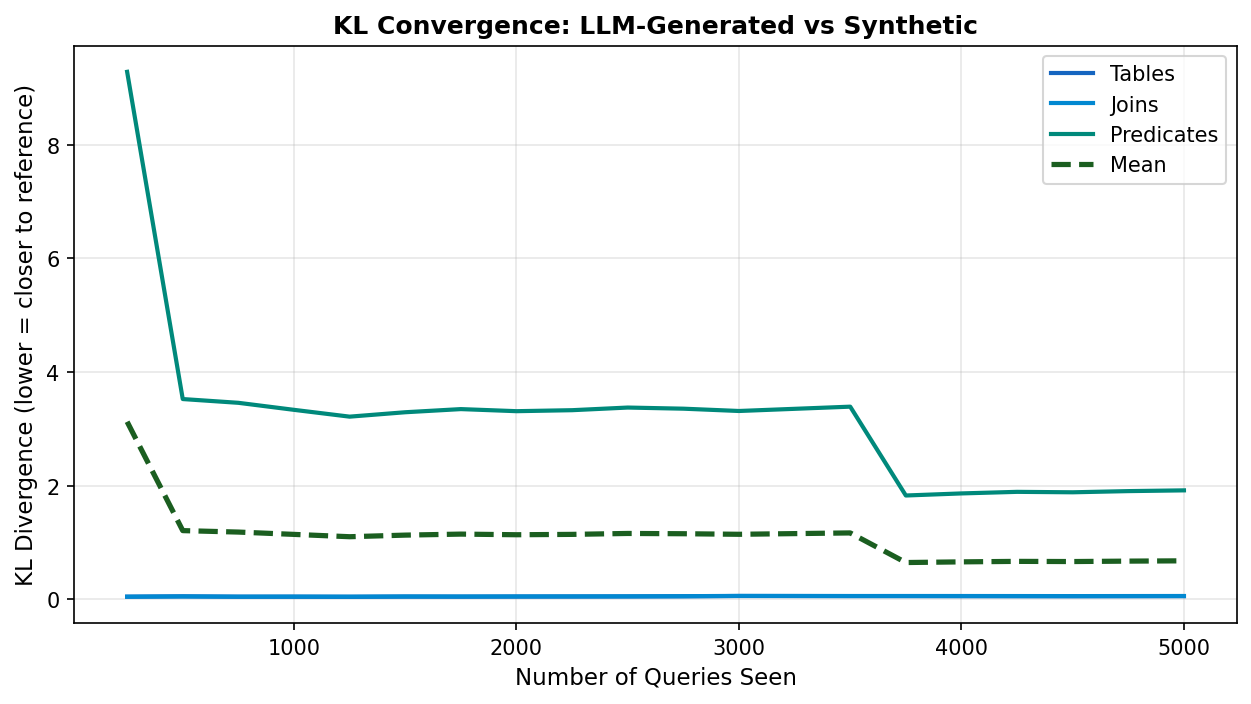
\includegraphics[width=0.9\textwidth]{kl_convergence.png}
\caption{KL-divergence convergence trends for tables, joins, predicates, and the aggregated mean between synthetic and LLM-generated workloads. Lower divergence values indicate stronger distributional similarity. The decreasing trends demonstrate progressive convergence toward the target workload characteristics as more queries are generated.}
\label{fig:kl_convergence}
\end{figure}

Figure~\ref{fig:kl_convergence} presents the KL-divergence trajectories for tables, joins, predicates, and the aggregated mean as the number of generated queries increases. Several important observations can be made from these convergence trends. A decreasing KL-divergence indicates that the generated workload distribution becomes increasingly similar to the target workload distribution over time. The table and join divergence curves remain near zero throughout the experiment and largely overlap visually due to their similarly low divergence values relative to the predicate distribution.

First, the divergence associated with table-count and join-count distributions decreases rapidly and stabilizes at relatively low values. This indicates that the LLM-generated workload successfully reproduces the overall structural composition of the reference workload, particularly with respect to query graph size and join complexity. The stability of these curves further suggests that the generation process does not collapse toward a narrow subset of repetitive query templates.

Second, predicate distributions exhibit higher divergence values compared to tables and joins. This behavior is expected because predicate generation involves greater combinatorial complexity. While table and join structures are constrained by the schema graph, predicate construction depends on combinations of columns, comparison operators, and value ranges, resulting in a significantly larger search space. Consequently, achieving convergence for predicate distributions requires a larger and more diverse query set.

Despite this increased variability, the predicate divergence demonstrates a clear downward trend as workload generation progresses. The aggregated mean KL divergence follows the same decreasing trajectory, indicating increasing similarity between the generated and reference workload distributions as additional queries are generated.

An important observation from Figure~\ref{fig:kl_convergence} is that divergence decreases more noticeably in the later stages of generation, after which the curves fluctuate within a lower range. This suggests that the workload generation process initially explores a broader structural space before gradually stabilizing around the target workload distribution. After this point, the divergence curves remain relatively stable, indicating that newly generated queries continue to preserve the desired workload characteristics rather than introducing excessive structural drift.

The convergence behavior observed in the KL-divergence analysis is particularly important for active learning. Active learning strategies rely on the availability of structurally diverse and statistically representative unlabeled samples. If the workload generation process produced highly repetitive or biased query structures, the acquisition function would repeatedly select similar queries, reducing the efficiency of uncertainty-driven sampling. The decreasing divergence trends therefore provide evidence that the generated workload maintains sufficient diversity while progressively aligning with the intended target distribution.

Overall, the KL-divergence analysis provides quantitative evidence that the proposed diversity-guided prompting strategy produces structurally stable and statistically representative workloads. Rather than repeatedly generating highly similar queries, the LLM progressively expands coverage across the workload feature space while maintaining alignment with the target structural distribution over time.

\begin{figure}[tb]
\centering
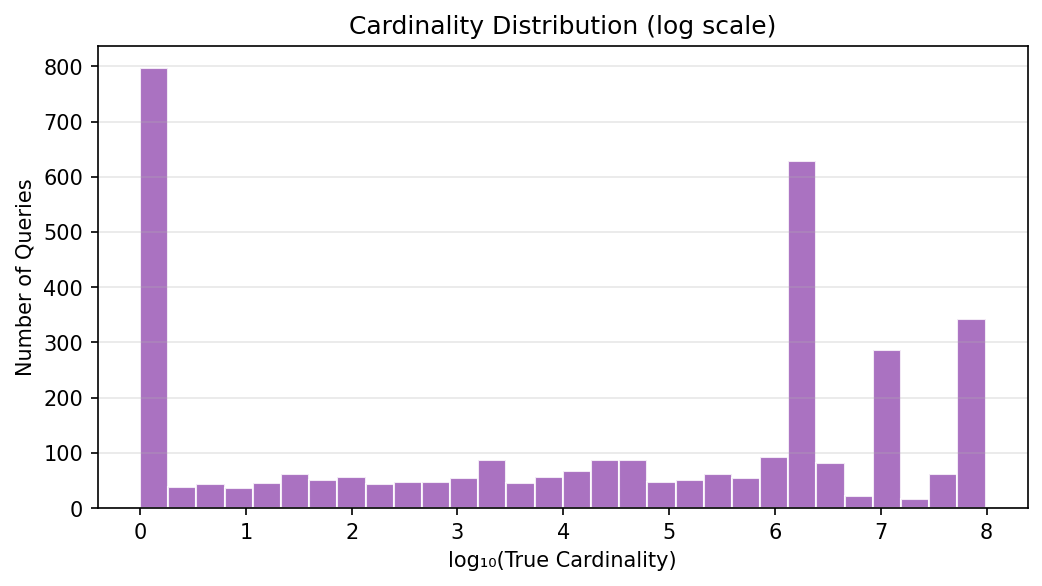
\includegraphics[width=0.85\textwidth]{data_cardinality_distribution.png}
\caption{Distribution of true query cardinalities on a logarithmic scale. The workload spans several orders of magnitude, exposing the estimator to both highly selective queries and large-scale scans.}
\label{fig:cardinality_dist}
\end{figure}

Finally, Figure~\ref{fig:cardinality_dist} shows the distribution of true query cardinalities on a logarithmic scale. The workload spans several orders of magnitude, ranging from highly selective queries returning only a few tuples to broad scans producing millions of rows. This long-tailed distribution is essential for training robust cardinality estimators, as it forces the model to learn accurate predictions across both sparse and dense selectivity regimes. The presence of such large variance also motivates the use of relative-error metrics such as Q-error, which remain meaningful across wide cardinality scales.

Overall, the workload analysis demonstrates that the generated query corpus captures substantial diversity across multiple orthogonal dimensions, including relational complexity, join structure, predicate composition, and selectivity behavior. This diversity is critical not only for supervised training but also for the effectiveness of active learning.

Furthermore, the convergence trends observed in the KL-divergence analysis suggest that the LLM-based generation process remains relatively stable as the workload grows. This is an important property for scalable workload generation because it indicates that increasing the query budget does not simply produce redundant templates, but instead incrementally improves coverage of the target workload distribution.

Taken together, these results validate the suitability of the generated workload for training learned cardinality estimators and provide empirical evidence that the proposed generation framework produces structurally rich and statistically representative query corpora.

\section{Active Learning and Model Training Results}

The workload diversity experiments presented in the previous section evaluate the structural properties of the LLM-generated query corpus. Due to the computational overhead associated with repeated query labeling and retraining, the controlled comparison between random sampling and MC Dropout acquisition strategies is conducted on synthetic workloads with predefined structural distributions.

In contrast, the subsequent labeling-efficiency and PostgreSQL comparison experiments are evaluated on LLM-generated workloads in order to assess the practical behavior of the proposed framework under automatically generated query distributions. This separation enables controlled analysis of active learning behavior while still evaluating the quality and executability of the LLM-generated workloads independently.

This section evaluates the effectiveness of the proposed active learning framework using workloads generated from synthetic query distributions. In particular, the experiments compare uncertainty-driven acquisition using MC Dropout against a standard random sampling baseline to determine whether uncertainty-aware query selection improves the efficiency, accuracy, and robustness of learned cardinality estimation.

The primary objective of active learning in this setting is to reduce the number of labeled training queries required to achieve strong estimation performance. Since obtaining query labels requires executing SQL queries against the underlying database system, labeling large workloads can be computationally expensive. An effective acquisition strategy should therefore identify the most informative queries for labeling, enabling the model to learn representative workload characteristics with fewer training samples.

The following analysis examines the learning behavior of the estimator across successive active learning rounds. In particular, we analyze convergence efficiency, prediction calibration, and the evolution of Q-error statistics under both random sampling and uncertainty-guided acquisition.

\subsection{Learning Efficiency Across Active Learning Rounds}

Figure~\ref{fig:learning_curve_comparison} compares the validation median Q-error achieved by random sampling and MC Dropout as the number of labeled synthetic queries increases. Both strategies exhibit a consistent reduction in validation error as additional labeled samples are incorporated into the training set, confirming that the estimator benefits from progressively larger workloads. However, the MC Dropout generally improves sample efficiency in this setup, but gains are not monotonic across rounds and can vary by run, seed, and workload sample.

\begin{figure}[tb]
\centering

\includegraphics[width=0.9\textwidth]{Report/graphs/comparison_learning_curves.png}
\caption{Learning curves comparing random sampling and MC Dropout on synthetic query workloads. MC Dropout consistently achieves lower validation median Q-error with the same labeling budget, indicating improved sample efficiency during query acquisition.}
\label{fig:learning_curve_comparison}
\end{figure}

The difference between the two acquisition strategies becomes increasingly pronounced during later rounds of active learning. While the improvement achieved by random sampling gradually begins to plateau, MC Dropout continues reducing validation error. These findings suggest that uncertainty-aware query selection can reduce the labeling effort required to train learned cardinality estimators while maintaining strong performance on the evaluated workloads.

An important observation is the final performance gap between the two strategies. MC Dropout achieves lower validation median Q-error while using the same labeling \textbf{budget as random sampling}, demonstrating improved sample efficiency. From an active learning perspective, this result supports the hypothesis that uncertainty estimates can guide the acquisition process toward queries that provide greater learning benefit than randomly selected samples.

Most performance improvement occurs during the early acquisition rounds, indicating that uncertainty-guided selection rapidly identifies highly informative queries. The persistent gap between MC Dropout and random sampling further suggests that uncertainty estimates remain useful in later training stages.

Figure~\ref{fig:mc_dropout_curve} further illustrates the convergence behavior of the MC Dropout strategy using a workload configuration with 1,000 labeled queries. The validation median Q-error decreases sharply during the initial acquisition rounds before gradually stabilizing as the model approaches convergence. Overall, the active learning process achieves approximately 71.7\% reduction in median validation Q-error relative to the initial model within this setting.

\begin{figure}[tb]
\centering
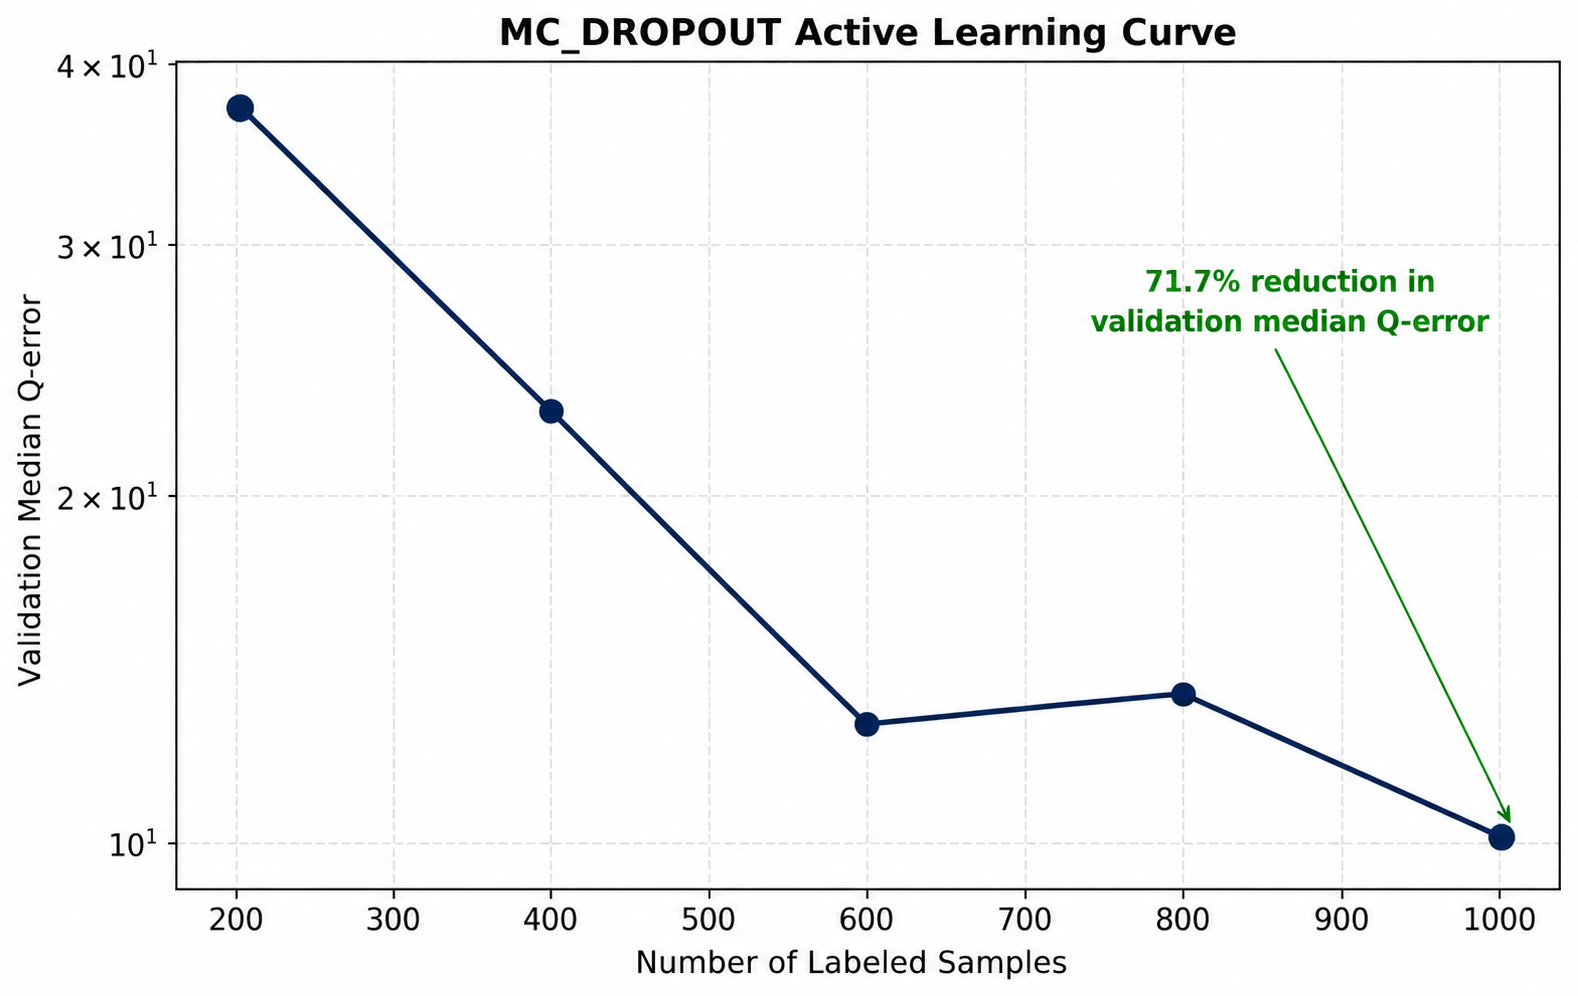
\includegraphics[width=0.75\textwidth]{train_learning_curve_mc_dropout.png}
\caption{MC Dropout active learning curve for the experimental configuration using 1,000 labeled queries. The reduction in validation median Q-error illustrates the convergence behavior of uncertainty-guided sample acquisition across active learning rounds.}
\label{fig:mc_dropout_curve}
\end{figure}

The steep decline during early rounds indicates that the model rapidly learns fundamental selectivity and join patterns from a relatively small set of informative synthetic queries before gradually approaching convergence.

\subsection{Prediction Accuracy and Calibration}

To evaluate prediction quality more directly, Figure~\ref{fig:predicted_vs_actual_comparison} compares predicted and actual cardinalities on a shared synthetic validation set. The plots are shown on logarithmic scales because query cardinalities span several orders of magnitude, ranging from highly selective queries to large-scale scans.

\begin{figure}[tb]
\centering

\includegraphics[width=\textwidth]{Report/graphs/comparison_predicted_vs_actual_scatter.png}
\caption{Predicted versus actual cardinalities for random sampling and MC Dropout on the shared synthetic validation set. Points closer to the diagonal line correspond to more accurate estimates. MC Dropout achieves tighter clustering around the diagonal and lower overall estimation error.}
\label{fig:predicted_vs_actual_comparison}
\end{figure}

Points located near the diagonal line correspond to accurate predictions, while deviations indicate estimation error. Both acquisition strategies successfully capture the overall trend of the validation workload, demonstrating that the MSCN estimator produces stable prediction behavior across multiple cardinality scales on the evaluated workload. However, the MC Dropout model exhibits visibly tighter clustering around the diagonal line, particularly for medium- and high-cardinality queries.

The reported median Q-errors further confirm this improvement. Random sampling achieves a median validation Q-error of 3.32, whereas MC Dropout reduces the median error to 2.77. This improvement suggests that uncertainty-guided acquisition improves estimation accuracy across the evaluated synthetic workload setup, demonstrating consistent gains over the baseline method.

Another important observation is that prediction dispersion increases toward the extreme ends of the cardinality spectrum. This behavior reflects the inherent difficulty of learned cardinality estimation, particularly for highly selective queries and extremely large joins where statistical correlations become increasingly difficult to model accurately. Despite these challenges, the MC Dropout strategy consistently produces estimates that remain closer to the ideal prediction line compared to the random baseline.

\subsection{Q-Error Distribution and Robustness Analysis}

While median Q-error provides a compact summary of estimation quality, analyzing higher-percentile errors provides additional insight into model robustness. Figure~\ref{fig:roundwise_qerror_stats} presents the evolution of median, 90th percentile (p90), and 95th percentile (p95) Q-errors across active learning rounds for both acquisition strategies. Lower median Q-error indicates improved average estimation quality, while reductions in upper-percentile errors indicate improved robustness against difficult outlier queries.

\begin{figure}[tb]
\centering

\includegraphics[width=0.95\textwidth]{Report/graphs/comparison_round_stats.png}
\caption{Round-wise validation Q-error statistics for random sampling and MC Dropout on synthetic workloads. The consistent reduction in median and tail-end errors demonstrates progressive improvement across active learning rounds.}
\label{fig:roundwise_qerror_stats}
\end{figure}

Several important trends emerge from this analysis. First, both acquisition strategies show substantial reductions in median Q-error as additional labeled queries are acquired over successive rounds. This confirms that active learning progressively improves the estimator’s ability to model workload selectivity patterns and join relationships.

Second, MC Dropout achieves consistently lower or comparable percentile errors across most rounds, particularly during later stages of training. The improvement is especially noticeable for the p90 and p95 metrics, which capture tail-end estimation behavior. 
Reducing extreme estimation errors is important because such failures can propagate through execution plans and negatively affect downstream optimization decisions.

Another important observation is the gradual stabilization of the percentile curves during later rounds. As the training workload becomes increasingly representative, the model approaches convergence and additional labeled queries provide smaller incremental improvements. This behavior is consistent with the convergence dynamics observed earlier in the learning curves.

The decreasing tail-end errors further indicate that uncertainty-guided acquisition improves not only average-case estimation quality but also robustness on difficult queries. By prioritizing uncertain or poorly modeled queries during acquisition, MC Dropout progressively reduces gaps in the model’s understanding of the workload distribution.

Overall, the experimental results demonstrate that MC Dropout provides a more effective active learning strategy than random sampling for synthetic query workloads. Compared to random acquisition, uncertainty-guided sampling achieves faster convergence, lower validation error, and stronger robustness across multiple evaluation metrics. These findings indicate that uncertainty-aware query selection improves sample efficiency and estimation robustness within the evaluated synthetic workload setting.

\section{Labeling Efficiency Analysis}

One of the primary motivations for incorporating active learning into the training pipeline is the high computational cost associated with obtaining query cardinality labels. Each labeled sample requires executing the corresponding SQL query against the database engine, which can become prohibitively expensive when training workloads contain thousands of queries. Consequently, reducing the number of required database executions is critical for improving the practical scalability of learned cardinality estimation systems.

The proposed active learning framework addresses this challenge by selectively labeling only the most informative queries rather than uniformly labeling the entire workload. Instead of treating all unlabeled queries as equally valuable, uncertainty-guided acquisition prioritizes samples that are expected to provide the greatest improvement to the estimator.

Figure~\ref{fig:labeling_efficiency} compares the labeling effort required by the active learning pipeline against a fully supervised baseline. The results demonstrate that the active learning approach achieves competitive estimation accuracy \textbf{while labeling only a fraction of the total query pool}. This reduction in labeling effort directly translates into lower execution overhead, reduced training time, and improved scalability for large workloads.

\begin{figure}[htbp]
\centering
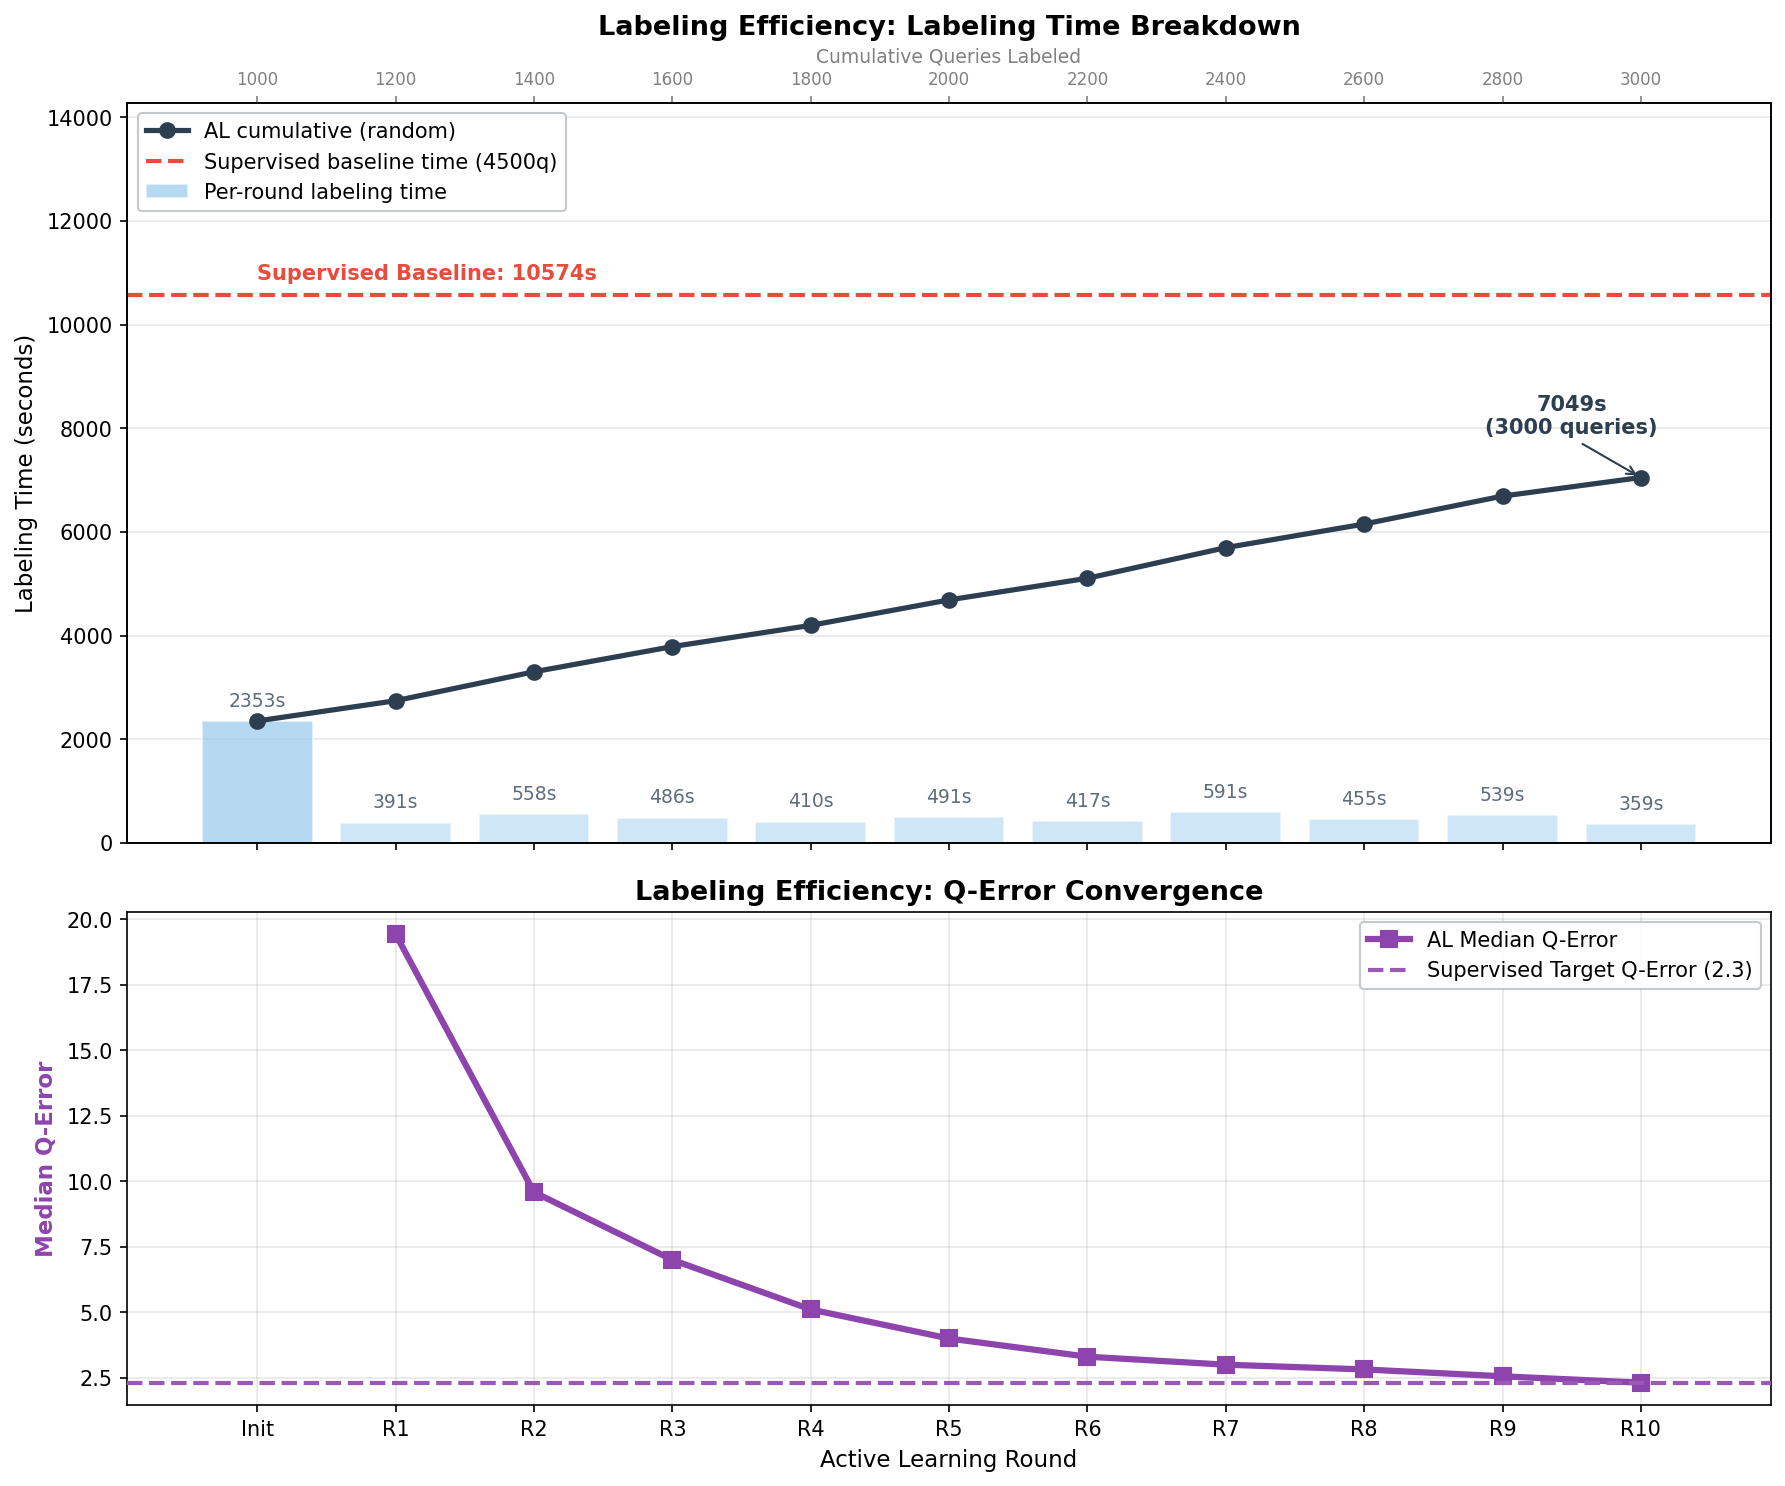
\includegraphics[width=\textwidth]{analysis_labeling_efficiency.png}
\caption{Labeling efficiency comparison between active learning and full supervision. The active learning framework achieves competitive estimation accuracy while requiring significantly fewer labeled queries, reducing the dominant execution cost in the training pipeline.}
\label{fig:labeling_efficiency}
\end{figure}

These results suggest that selectively labeling informative queries provides substantially greater learning benefit than uniformly expanding the labeled workload. By focusing labeling resources on uncertain or poorly modeled queries, the active learning framework extracts substantially more learning value per database execution than random or exhaustive labeling approaches.

This improvement is particularly important for learned cardinality estimation because workload labeling is often the dominant computational bottleneck in the training pipeline. Large analytical queries may require substantial execution time, especially when generating workloads spanning diverse join structures and selectivity conditions. Reducing the number of required executions therefore improves not only computational efficiency but also the practical feasibility of retraining estimators as database contents evolve over time.

Figure~\ref{fig:labeling_rate} further analyzes the robustness of the labeling pipeline by reporting the proportion of generated queries that were successfully labeled within the configured execution constraints.

\begin{figure}[htbp]
\centering
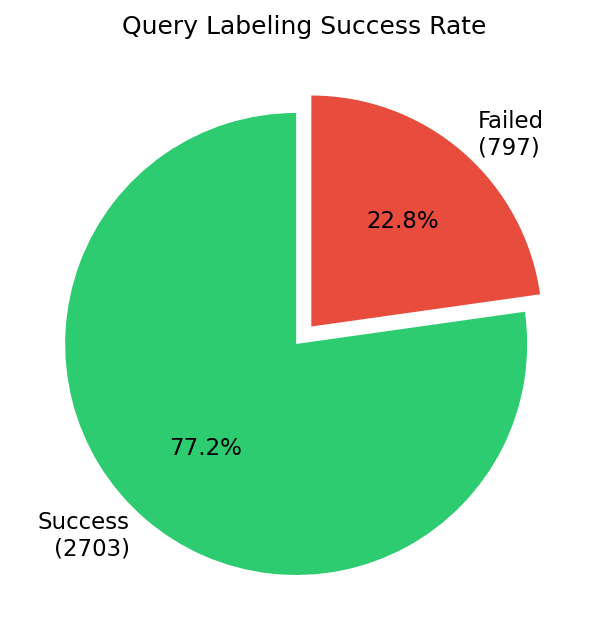
\includegraphics[width=0.85\textwidth]{analysis_labeling_rate.png}
\caption{Queries exceeding timeout limits or failing after retries are retained using a fallback cardinality value, so the pipeline can continue without dropping samples. As a result, the labeling outcome should be interpreted as successful executions versus fallback-labeled cases, not strict inclusion versus exclusion. The high success rate demonstrates that the generated queries remain largely executable within practical execution constraints.}
\label{fig:labeling_rate}
\end{figure}

Queries that exceed the database timeout threshold or repeatedly fail during execution are excluded from the final labeled workload. Such failures may arise from excessively expensive join plans, execution instability, or resource limitations within the database system. Despite these challenges, the labeling pipeline achieves a high overall success rate, indicating that the generated LLM workloads remain largely executable within realistic execution limits.

The high labeling success rate also provides indirect evidence that the workload generation framework produces largely executable queries. Since the generated queries are overwhelmingly executable and produce valid cardinality labels, the diversity-guided prompting strategy successfully balances structural complexity with practical executability. This balance is essential because excessively complex or pathological queries would reduce labeling throughput and limit the usefulness of the generated workload for active learning.

Overall, the labeling efficiency analysis demonstrates that active learning substantially reduces the execution cost associated with workload labeling while maintaining strong estimator performance. These results suggest that uncertainty-guided query acquisition can reduce labeling cost while maintaining strong estimation performance on diverse query workloads.

\section{Comparison with PostgreSQL Optimizer}

To further evaluate the effectiveness of the learned estimator, we compare its cardinality predictions directly against those produced by PostgreSQL’s native query optimizer. PostgreSQL relies primarily on histogram statistics and independence assumptions when estimating query cardinalities, whereas the MSCN model learns statistical relationships directly from query workloads and execution results.

This comparison is particularly important because cardinality estimation quality directly influences downstream query optimization decisions, including join ordering, operator selection, and memory allocation. Even moderate estimation errors can propagate through execution plans and significantly degrade query performance. Consequently, demonstrating improvements over the native PostgreSQL estimator provides evidence of the effectiveness of the proposed learned approach on the evaluated workload.

Figure~\ref{fig:pg_line} compares the distribution of Q-error values across query quantiles for PostgreSQL and the MSCN estimator on the shared validation workload. The evaluation in this section is conducted on the LLM-generated validation workload described earlier in the chapter.

\begin{figure}[tb]
\centering

\includegraphics[width=\textwidth]{Report/graphs/compare_pg_vs_mscn_qerror_line.png}
\caption{Q-error by query quantile for PostgreSQL and the MSCN estimator on the validation workload. Lower curves indicate more accurate cardinality estimates across the evaluated query distribution, while steep increases near the upper quantiles reflect difficult outlier queries with large estimation errors.}
\label{fig:pg_line}
\end{figure}

The percentile-based comparison reveals substantially different error characteristics between the two estimators. PostgreSQL maintains relatively low Q-error values across most of the workload but exhibits extremely large estimation failures in the highest query quantiles, where Q-error increases abruptly by several orders of magnitude. In contrast, the MSCN estimator produces higher median error throughout much of the distribution but avoids the catastrophic outlier behavior observed in PostgreSQL. This suggests that the learned estimator achieves more stable worst-case behavior while sacrificing some accuracy on simpler query instances.

The sharp error escalation near the upper quantiles highlights structurally difficult queries involving highly selective predicates, sparse joins, or complex correlation patterns. Such queries challenge traditional histogram-based estimators because estimation errors propagate multiplicatively across join operations. The smoother MSCN error profile indicates more consistent generalization under these challenging conditions, even though its average estimation accuracy remains less competitive on easier portions of the workload.
\begin{figure}[tb]
\centering

\includegraphics[width=\textwidth]{compare_pg_vs_mscn_scatter.png}
\caption{Predicted versus actual cardinalities for PostgreSQL and MSCN. Points closer to the diagonal line correspond to more accurate cardinality estimates.}
\label{fig:pg_scatter}
\end{figure}

Across most query percentiles, PostgreSQL achieves lower Q-error than the MSCN estimator, indicating more accurate cardinality estimates for a large portion of the evaluated workload overall. This behavior is expected because the evaluated queries largely follow relatively simple predicate and join structures that align well with PostgreSQL’s histogram-based estimation framework. However, PostgreSQL also exhibits severe estimation failures in the highest query quantiles, whereas the MSCN estimator produces a comparatively smoother error profile with fewer catastrophic outliers. These results suggest that the learned estimator captures workload-dependent correlations and selectivity patterns that are difficult to represent using traditional histogram-based estimation methods alone.

The advantage of the MSCN estimator becomes particularly important for complex multi-table queries and highly selective predicates, where traditional independence assumptions often break down in practice. By learning representations directly from workload behavior, MSCN is able to model dependencies between predicates and joins more effectively than traditional histogram-based estimation methods.

Figure~\ref{fig:pg_scatter} provides visualization by comparing predicted and actual query cardinalities on a logarithmic scale. Points located near the diagonal line correspond to accurate predictions, while larger deviations indicate estimation error.

The MSCN predictions exhibit a comparatively smoother distribution of estimation errors across different cardinality ranges, while PostgreSQL demonstrates larger deviations for a small subset of difficult queries. These difficult cases are likely associated with correlated predicates or sparse join patterns that are challenging for traditional histogram-based estimation methods.

Another important observation is that the learned estimator maintains improved accuracy even at the extremes of the cardinality spectrum. Estimating very small or very large cardinalities is particularly challenging because such queries often correspond to sparse or highly correlated regions of the workload distribution. The improved stability of MSCN in these regions demonstrates the benefit of workload-driven learning for capturing complex statistical relationships.

Overall, the comparison with PostgreSQL demonstrates that traditional histogram-based estimation remains highly effective for a large portion of the evaluated workload, particularly for simpler query structures and predicates. However, the learned MSCN estimator exhibits more stable behavior on difficult outlier queries and complex selectivity patterns where traditional independence assumptions become less reliable. These results suggest that workload-driven learned estimators can complement traditional optimizer statistics, particularly for challenging query distributions involving sparse joins and correlated predicates.

\section{Discussion}

This chapter evaluated the proposed active learning framework across multiple dimensions, including workload diversity, labeling efficiency, estimation accuracy, and robustness. The experimental results demonstrate that the proposed framework produces structurally diverse LLM-generated query workloads and that uncertainty-guided acquisition improves learning efficiency on the evaluated synthetic workloads.

Beyond the quantitative improvements observed in validation Q-error and workload coverage, the experiments also provide broader insights into the behavior of learned cardinality estimation systems and the practical trade-offs involved in building scalable data-driven query optimizers. 

\subsection{Active Learning and Workload Diversity}

The experimental results demonstrate that uncertainty-guided acquisition improves labeling efficiency by prioritizing informative queries rather than uniformly sampling the workload. Queries associated with high predictive uncertainty typically correspond to regions of the workload distribution that are underrepresented or poorly modeled by the current estimator.

The learning curves indicate rapid improvement during early acquisition rounds followed by gradual convergence as the estimator observes increasingly representative workload patterns.

An important implication of these findings is that query quality is more important than query quantity during training. A relatively small but carefully selected labeled workload can provide comparable learning benefit to substantially larger randomly labeled datasets. This observation highlights the practical value of uncertainty-guided acquisition for reducing database execution overhead while maintaining strong estimation accuracy.

The quality of a learned cardinality estimator depends heavily on the diversity of the workload used during training. If the workload contains highly repetitive query structures or narrow selectivity patterns, the estimator may overfit to a limited subset of query templates and fail to generalize to unseen workloads.

The workload generation strategy proposed in this thesis addresses this challenge through diversity-guided prompting and structural constraint mechanisms. Rather than generating queries independently without feedback, the LLM is continuously guided using workload statistics such as table counts, join distributions, predicate frequencies, and cardinality ranges.

The workload analysis indicates that the proposed generation framework maintains broad workload coverage while progressively converging toward the target workload distribution. This balance between diversity and distributional stability is particularly important for active learning because it provides heterogeneous unlabeled samples without collapsing toward repetitive query templates.

An important observation from the KL-divergence analysis is that predicate distributions converge more slowly than join or table distributions. A likely explanation is that predicate construction involves significantly greater combinatorial complexity. While table and join structures are constrained by the schema graph, predicates depend on combinations of columns, operators, and value ranges, resulting in a much larger structural search space.

Despite this increased variability, the workload generation process avoids collapsing toward overly repetitive query structures. This behavior is particularly important because active learning fundamentally relies on the availability of sufficiently diverse unlabeled samples for effective learning. If the generated workload lacked sufficient structural variation, the acquisition process would provide only limited additional information in later rounds, thereby reducing its overall effectiveness.

The results therefore reinforce the importance of workload diversity for learned cardinality estimation. The value of LLM-based workload generation lies not only in automating SQL query creation but also in enabling broader structural exploration than would be feasible using manually designed templates alone.

\subsection{Practicality and Scalability of the Pipeline}

Another important contribution of this work is the development of a fully automated pipeline for workload generation, labeling, and model training. Traditional workload construction often requires significant manual effort, including hand-written query templates, schema-specific heuristics, and extensive tuning for each database environment.

The proposed framework reduces this manual dependency by leveraging LLM-guided workload generation combined with automated validation and labeling stages. Because the pipeline relies primarily on schema metadata and workload statistics, it remains largely schema-independent within the supported query fragment and adaptable to relational schemas with defined join relationships.

The modular architecture of the system also improves reproducibility and experimentation efficiency. Individual components such as workload generation, query validation, uncertainty acquisition, labeling, and training can be modified independently without redesigning the entire pipeline. This flexibility simplifies experimentation with alternative acquisition strategies, model architectures, and workload configurations.

Another practical advantage is the reduction in engineering overhead associated with maintaining manually curated query workloads. Once schema information is extracted, the pipeline can continuously generate new training queries with minimal human intervention. This capability becomes increasingly valuable in dynamic environments where workloads evolve over time and estimators require periodic retraining.

The high query validation and labeling success rates observed during experimentation further demonstrate that the automated generation strategy successfully balances workload diversity with practical executability. The majority of generated queries remain executable within the configured timeout limits, indicating that the workload generation process generally avoids excessively expensive query structures.

Although active learning improves labeling efficiency, it also introduces additional computational overhead compared to traditional supervised learning pipelines. In particular, uncertainty estimation using MC Dropout requires multiple stochastic forward passes through the model during acquisition. This increases inference cost relative to random query selection.

Another source of overhead arises from workload preprocessing and bitmap generation. The MSCN representation relies on sampled bitmap features to capture predicate selectivity information, and generating these features requires additional preprocessing during workload construction.

However, the experimental results suggest that these overheads are acceptable relative to the cost of exhaustive query labeling. Database execution remains the dominant computational bottleneck in the pipeline, particularly for complex analytical queries involving multi-way joins and large cardinalities. Reducing the number of required labeled queries therefore provides substantially greater computational savings than the additional inference cost introduced by uncertainty estimation.

An important trade-off also exists between workload diversity and execution efficiency. More structurally diverse workloads improve estimator generalization but may also increase the probability of generating expensive or difficult-to-execute queries. The validation and timeout filtering stages are therefore essential for ensuring that the final workload remains practically executable while preserving sufficient structural diversity.

Overall, the results suggest that uncertainty-guided active learning provides a balance between computational overhead and labeling efficiency. The additional acquisition cost introduced by MC Dropout is outweighed by the reduction in expensive database executions required to train an accurate estimator.

\subsection{Sources of Estimation Error}

Despite the overall improvement achieved by the learned estimator, several sources of estimation error remain challenging. One major difficulty arises from highly selective queries and extremely large joins, where sparse or skewed data distributions make accurate estimation inherently difficult.

Another important challenge involves unseen predicate combinations and rare join patterns that are poorly represented within the training workload. Although the diversity-guided generation strategy improves structural coverage, it is still difficult to exhaustively explore the enormous combinatorial space of possible SQL queries.

Prediction errors may also arise from limitations of the sampled bitmap representation used by MSCN. Bitmap samples provide only an approximate representation of predicate selectivity and may fail to capture fine-grained correlations within highly skewed datasets.

Workload shift represents an additional challenge for learned estimators. If the query distribution observed during deployment differs substantially from the workload used during training, model accuracy may degrade due to insufficient generalization. This limitation is particularly relevant in evolving database environments where application behavior changes over time.

Finally, the current workload generation framework focuses primarily on selection and join queries with relatively constrained SQL structure. More advanced SQL constructs such as nested subqueries, aggregations, window functions, and complex expressions are not extensively explored in the current implementation. Supporting these constructs would likely require more sophisticated workload generation and representation techniques.

\subsection{Implications for Learned Query Optimization}

The comparison with PostgreSQL highlights several important differences between learned and traditional cardinality estimation approaches. PostgreSQL primarily relies on histogram statistics, selectivity heuristics, and attribute independence assumptions when estimating query cardinalities.

While these techniques are computationally efficient, they often struggle to model correlations between predicates and joins, particularly for complex analytical workloads. As query complexity increases, estimation errors may accumulate throughout the execution plan and negatively affect downstream optimization decisions.

The experimental comparison suggests that workload-driven learned estimators are better able to capture complex predicate and join correlations than traditional statistics-based approaches on the evaluated workload. On the evaluated workload, PostgreSQL achieves lower Q-error over much of the distribution, while MSCN shows smoother tail behavior with fewer catastrophic outliers on difficult queries.

These findings suggest that workload-driven learned estimators can complement traditional query optimization pipelines, particularly in environments where complex workload correlations are difficult to capture using classical statistics.

The findings of this thesis have broader implications for the development of learned database systems and adaptive query optimizers. The results demonstrate that learned cardinality estimation can benefit substantially from automated workload generation and uncertainty-guided acquisition strategies.

One important implication is that the practical training cost of learned estimators depends not only on model architecture but also on the efficiency of the data acquisition process. Active learning provides a practical mechanism for reducing the dominant labeling cost while preserving estimator quality.

The integration of LLM-based workload generation further expands the feasibility of learned optimization pipelines by reducing the manual effort traditionally required to construct representative training workloads. As language models continue improving, automated workload generation may become increasingly capable of producing structurally diverse query distributions with minimal human supervision.

More broadly, the combination of learned estimation, uncertainty-guided acquisition, and automated workload generation illustrates how automated workload generation and adaptive acquisition strategies could support more self-adaptive learned database components capable of adapting continuously to evolving workloads. Such systems could dynamically acquire informative queries, retrain estimation models, and potentially improve optimization quality over time without requiring extensive manual intervention.

Overall, the results indicate that integrating automated workload generation with uncertainty-guided acquisition provides a practical framework for improving the scalability and labeling efficiency of learned cardinality estimation.

\section{Limitations and Threats to Validity}

Several limitations should be considered when interpreting the results presented in this thesis.

First, all experiments in this study were performed on the IMDB benchmark schema within a PostgreSQL environment. Although the proposed pipeline is designed to be largely schema-independent within the supported query fragment, the observed results may not directly generalize to substantially different schemas, database systems, or workload characteristics without additional evaluation.

Another limitation concerns workload realism. While the LLM-generated workloads exhibit structural diversity across joins, predicates, and selectivity ranges, they may not fully reflect real-world production query distributions. The generated workloads primarily consist of analytical \texttt{SELECT COUNT(*)} queries with constrained SQL structure and therefore do not capture the full complexity of operational database workloads.

The current implementation also focuses specifically on the MSCN architecture. Different learned cardinality estimation models may interact differently with active learning strategies and synthetic workload generation. As a result, the observed improvements cannot necessarily be assumed to transfer directly to alternative neural architectures without further experimentation.

Several practical constraints within the labeling pipeline may additionally influence the results. Ground-truth labels were obtained through database execution using timeout constraints and retry mechanisms. Queries exceeding the configured execution limits may either fail labeling or be retained with fallback labels, depending on the labeling path used. This can introduce label noise and should be considered when interpreting model accuracy and robustness. Similarly, bitmap-based representations provide only an approximate view of predicate selectivity and may not fully capture complex correlations or highly skewed data distributions.

Another important limitation concerns evaluation scope. The experiments primarily evaluate cardinality estimation quality using Q-error metrics. Although improved cardinality estimates are generally associated with better query optimization decisions, the experiments do not directly measure downstream effects on execution-plan quality, join ordering, or end-to-end query latency.

Finally, due to computational constraints, experiments were conducted using single training runs for each configuration. Neural network training and active learning may exhibit variability across random seeds and workload sampling processes. Future work should therefore evaluate the statistical robustness of the observed improvements across repeated experimental trials.
% !TEX root =  main.tex
\chapter{Conclusion}
\label{chap:conclusion}
\pagestyle{plain}

\section{What We Built and What We Learned}

This thesis set out to answer a practical question: can we train a cardinality estimator well while keeping the number of expensive database executions manageable? The answer, based on our experiments, is yes. By combining LLM-based query generation with active learning, we built a pipeline that reaches competitive estimation accuracy using a fraction of the labels that a fully supervised approach would require.

Several pieces had to come together to make this work. The LLM-based generator, guided by structured prompts and diversity hints, produced workloads with enough variety in join patterns, predicate types, and selectivity profiles to give the model broad coverage of the query space. The four-layer validation filter caught the inevitable mistakes hallucinated columns, forbidden keywords and malformed syntax before they could corrupt the training data. And the active learning loop, particularly with Monte Carlo dropout as the acquisition function, proved effective at steering the labeling budget toward the queries that mattered most.

The result is a schema-agnostic, end-to-end system. Point it at a new database, give it a schema file, and it generates queries, validates them, labels the most informative ones, trains the estimator, and produces a diagnostic dashboard all without manual intervention.

The experimental evaluation further demonstrated that uncertainty-guided acquisition can reduce labeling requirements compared to uniform sampling while maintaining competitive estimation accuracy. More broadly, the results indicate that combining automated workload generation with active learning provides a practical and scalable approach for training learned cardinality estimation systems under limited labeling budgets.


\section{Limitations}

The proposed framework currently supports only conjunctive \texttt{SELECT COUNT(*)} queries containing AND-connected comparison predicates over numeric columns. More complex SQL constructs, including \texttt{OR} conditions, subqueries, \texttt{GROUP BY} clauses, and string-based predicates, are not supported by the current MSCN feature representation. Extending the framework to handle richer SQL fragments would require modifications to both the feature extraction pipeline and the prompt generation constraints.

The experiments were conducted on a single benchmark dataset (IMDB). While the pipeline is schema-agnostic by design, we have not yet verified how well the trained models generalize across different data distributions or schema structures. A retail database with skewed foreign key distributions might pose challenges that IMDB does not.

Monte Carlo dropout adds computational overhead. Running twenty-five forward passes per query per round is acceptable when the alternative is executing that query on a database, but for very large unlabeled pools the scoring step can become a bottleneck. Batch-level approximations or learned acquisition functions could help.

Finally, query execution failures still reduce the number of usable training
samples. Although the fraction of failed queries remains relatively small in the
current experiments, schemas containing more complex joins or larger data
volumes could increase the number of discarded queries and therefore reduce
labeling efficiency.


\section{Future Work}

The most natural next step is extending the query fragment. Supporting disjunctions, \texttt{LIKE} predicates, and basic aggregations would make the estimator applicable to a much wider range of real workloads. This would require rethinking the encoding scheme, but the rest of the pipeline generation, validation, active learning would carry over with relatively minor modifications.

Cross-schema transfer is another promising direction. If a model trained on IMDB could be fine-tuned for a retail database using only a handful of labels, the practical value of the system would increase substantially. Meta-learning and domain adaptation techniques are worth exploring here.

On the active learning side, combining uncertainty with diversity selecting queries that are both individually uncertain and collectively cover different parts of the feature space could improve sample efficiency further. Multi-objective acquisition functions that balance exploration, exploitation, and computational cost are a natural fit.

From a systems perspective, integrating the learned estimator into a live query optimizer and measuring the end-to-end impact on query execution time would close the loop between estimation accuracy and actual system performance. The current evaluation uses Q-error as a proxy, but what ultimately matters is whether better estimates lead to better plans.
  
\bibliographystyle{plain}
\bibliography{main}

\end{document}
